 La velocidad del viento es una magnitud vectorial tridimensional que experimenta fluctuaciones aleatorias de pequeña escala en el espacio y en el tiempo, que se superponen a un flujo organizado de mayor escala. Para los fines de la observación meteorológica, la meteorología sinóptica y el pronóstico del tiempo, es crucial analizar el movimiento horizontal del aire. No obstante, es importante considerar que, para algunas aplicaciones, también es necesario conocer el movimiento vertical del viento. Ejemplos de esto son el aterrizaje de aeronaves y el estudio de la dispersión de contaminantes en la atmósfera. En la Figura \ref{fig:vectorVelocidad} se muestran las tres componentes de un vector de viento $\mathbf{v_{xyz}}$, y sobre el plano $XY$ se muestra la proyección $\mathbf{v_{xy}}$ que nos interesa analizar.

\begin{figure}[H]
    \centering
    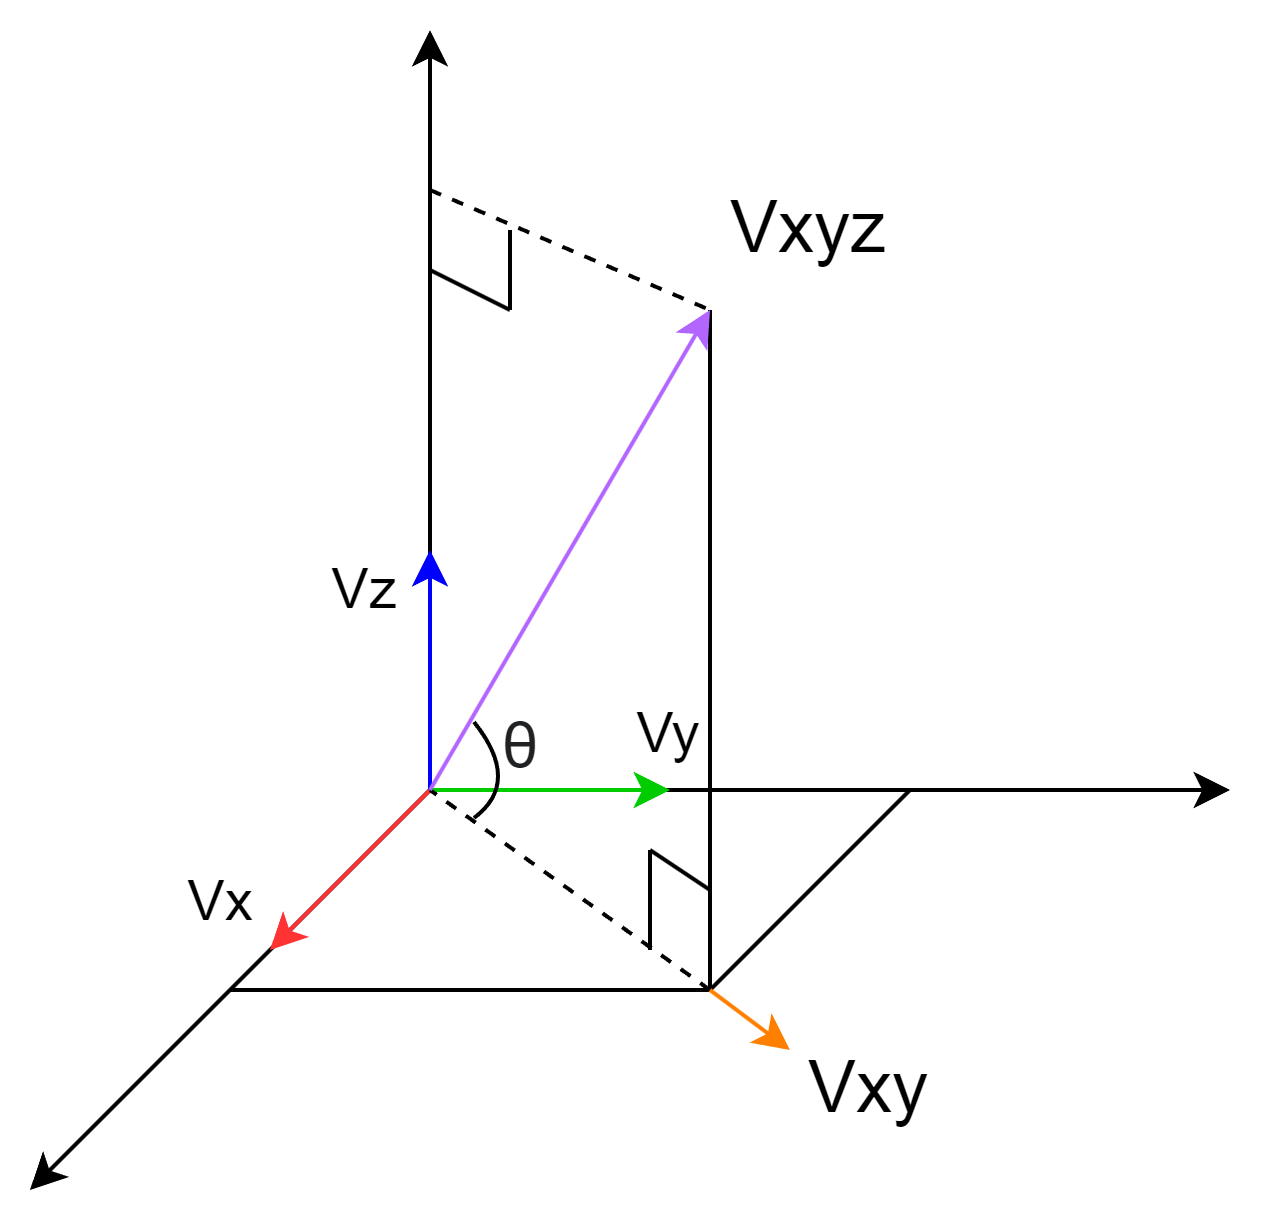
\includegraphics[width=0.5\linewidth]{Figuras/introduccion/vectorVelocidad.png}
    \caption{Tres componentes de la velocidad de viento $v_{x}, v_{y}, v_{z}\  [\unit{\meter\per\second}]$. El vector de viento horizontal $v_{xy}$ forma un ángulo de entrada $\theta$ con el vector de viento resultante $v_{xyz}$.} 
    \label{fig:vectorVelocidad}
\end{figure}
%%%%%%%%%%%%%%%%%%%%%%%%%%%%%%%%%%%%%%%%%%%%%%%%%%%%%%%%%%%%%%%%%%%%%%%%%%%%%%%%%%%%%%%%%%%%%%%%%%%%%%%%%%%%%%%%%%%%%%%%
\section{Viento en superficie}\label{sec:vientoEnSuperficie}
Se considerará que el viento de superficie es fundamentalmente una magnitud vectorial bidimensional definida por dos componentes
\begin{itemize}
    \item \textbf{Intensidad:} Indica el valor de la velocidad del viento. En general se utilizan unidades como nudos (\unit{\knot}), metros por segundo (\unit{\meter\per\second}) o kilómetros por hora (\unit{\kilo\meter\per\hour}).
    \item \textbf{Dirección y sentido:} Indica desde donde proviene el aire que se encuentra en movimiento. Se mide en grados sexagesimales y considera el apartamiento con respecto al norte geográfico. Por ejemplo, un viento de dirección noreste (aire que se desplaza del noreste hacia el suroeste) tiene una dirección de 45°, ya que esta es la separación (en grados) entre el norte y el noreste.
\end{itemize}

El grado de fluctuación experimentado por el viento se denomina  rafagosidad, y las diferentes fluctuaciones son conocidas como ráfagas o rachas. La mayoría de los usuarios de datos sobre el viento necesitan conocer el viento horizontal en promedio, eliminando las fluctuaciones. Por ejemplo, en meteorología se utilizan promedios de entre 10 y 60 minutos con fines de predicción, mientras que en aeronáutica se utilizan promedios de 2 minutos. No obstante, cada vez son más las aplicaciones que precisan información acerca de la variabilidad o rafagosidad del viento. Para este propósito, se utilizan tres magnitudes: la ráfaga o racha máxima, y las desviaciones típicas de la velocidad y de la dirección del viento \cite{wmoChapter8}. La representación gráfica del viento se puede realizar de distintas formas, entre ellas se encuentran las flechas, las barbas y las líneas de corriente. Las \textbf{flechas} \cite{CursoDeObsevadores} son la forma más común de representar un vector. La intensidad del viento se representa con la longitud de la flecha, mientras que la dirección se indica por el ángulo respecto al norte. El sentido de la flecha siempre apunta "hacia dónde va el viento". En la Figura \ref{fig:mapaFlechas} se muestra un ejemplo en el que se observa que el viento en la Patagonia proviene principalmente del sector oeste (es decir, el aire se desplaza de oeste a este), por lo tanto, las flechas apuntan hacia el este.

\begin{figure}[H]
    \centering
    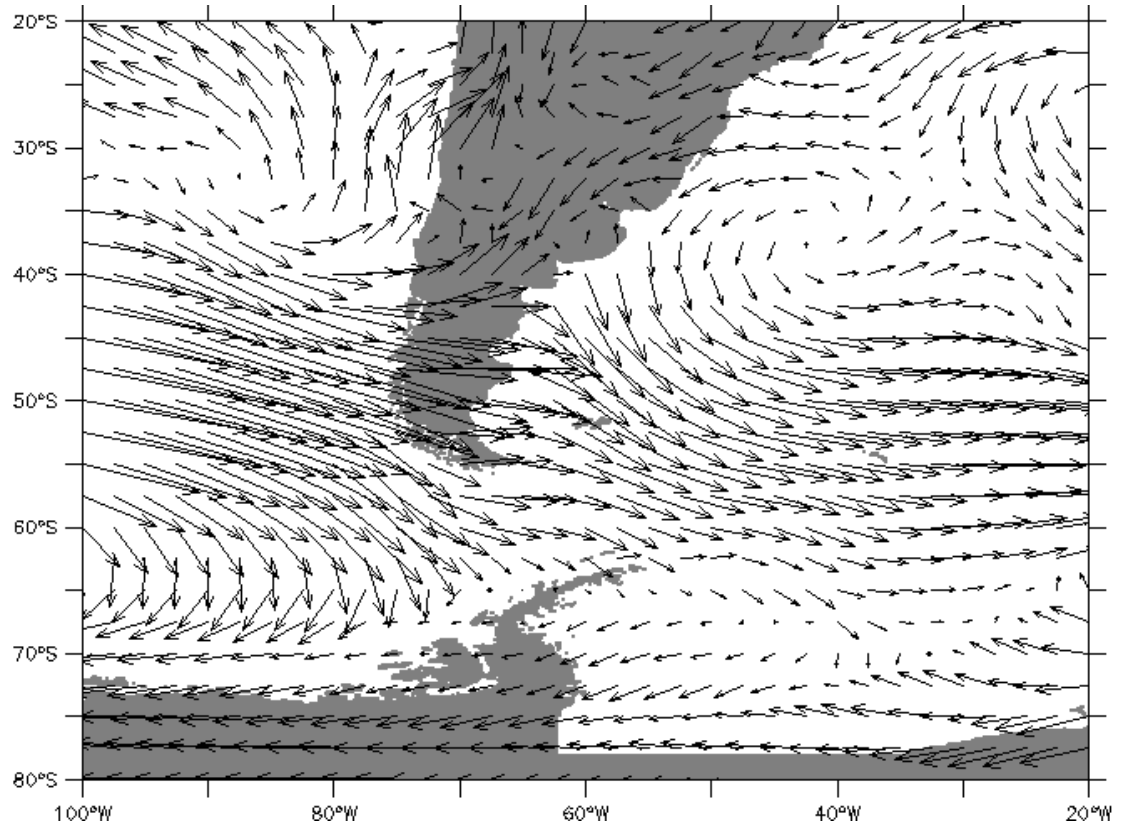
\includegraphics[width=0.85\linewidth]{Figuras/viento/mapaFlechas.png}
    \caption{Campo de viento representado con flechas en el sur de Sudamérica \cite{cursoObservadores2024}. }
    \label{fig:mapaFlechas}
\end{figure}

Las \textbf{barbas} \cite{CursoDeObsevadores} son ideogramas en los que la línea más larga indica la dirección del viento, mientras que las líneas más pequeñas, ubicadas en un extremo, indican la intensidad en múltiplos de 5 nudos. En la Figura \ref{fig:barbas1}, a izquierda, se puede observar una representación del viento del oeste con una intensidad de 15 nudos, donde la media flecha representa 5 nudos y la flecha entera representa 10 nudos. En el centro, se observa una barba que representa el viento del sur con un banderín negro que indica una intensidad de 50 nudos. Más a la derecha se observa una barba que representa el viento proveniente del sureste con una intensidad dada por un banderín, dos líneas largas y una media linea, en total suman 75 nudos. La dirección del viento está dada por el ángulo respecto al norte verdadero y, como se mencionó anteriormente, indica desde dónde viene el aire.

\begin{figure}[H]
    \centering
    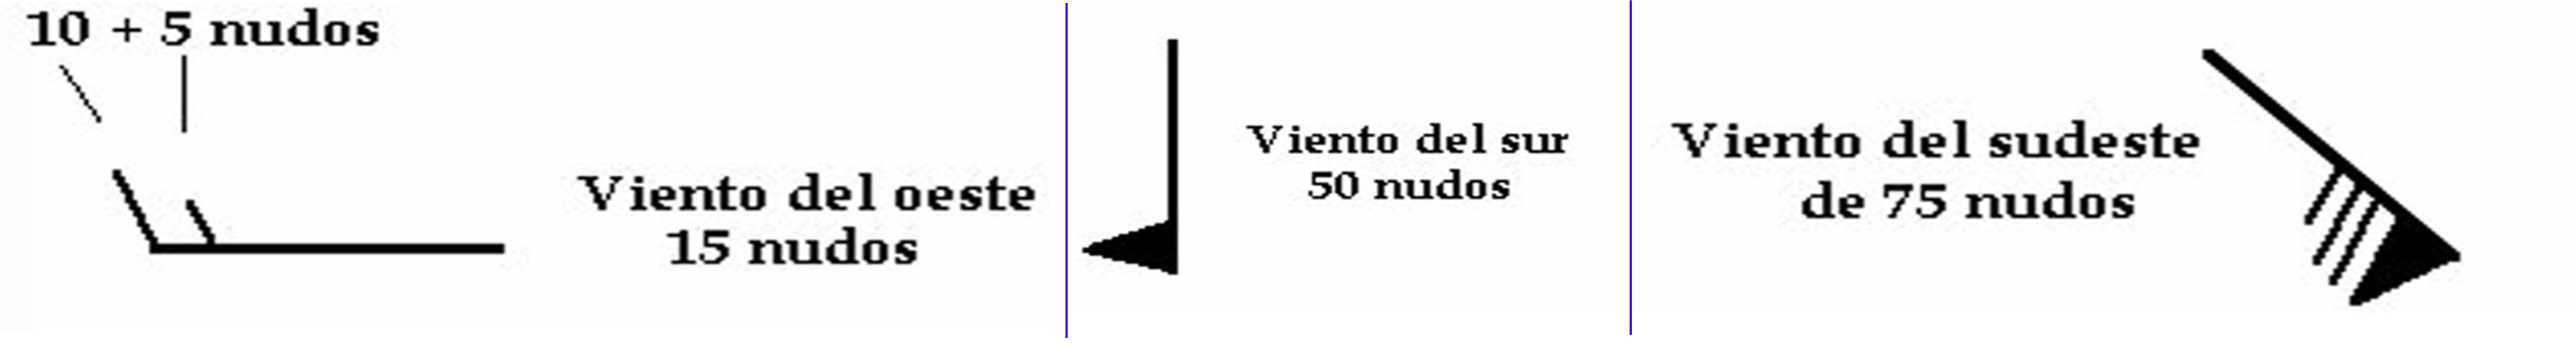
\includegraphics[width=1\linewidth]{Figuras/viento/barbas.png}
    \caption{Representación gráfica del viento utilizando barbas \cite{cursoObservadores2024}.}
    \label{fig:barbas1}
\end{figure}

Las barbas son ampliamente utilizadas en meteorología sinóptica y aeronáutica. En la Figura \ref{fig:mapaBarbas} se muestra una representación gráfica del viento en 850 \unit{\hecto\pascal} utilizada en la meteorología aeronáutica. Nótese que en la elipse roja inferior, el viento es de 40 nudos proveniente del sector oeste en el norte de la Patagonia, mientras que en la zona central del país, en la elipse roja superior, prevalecen vientos del sector norte en torno a los 10 y 15 nudos.


\begin{figure}[H]
    \centering
    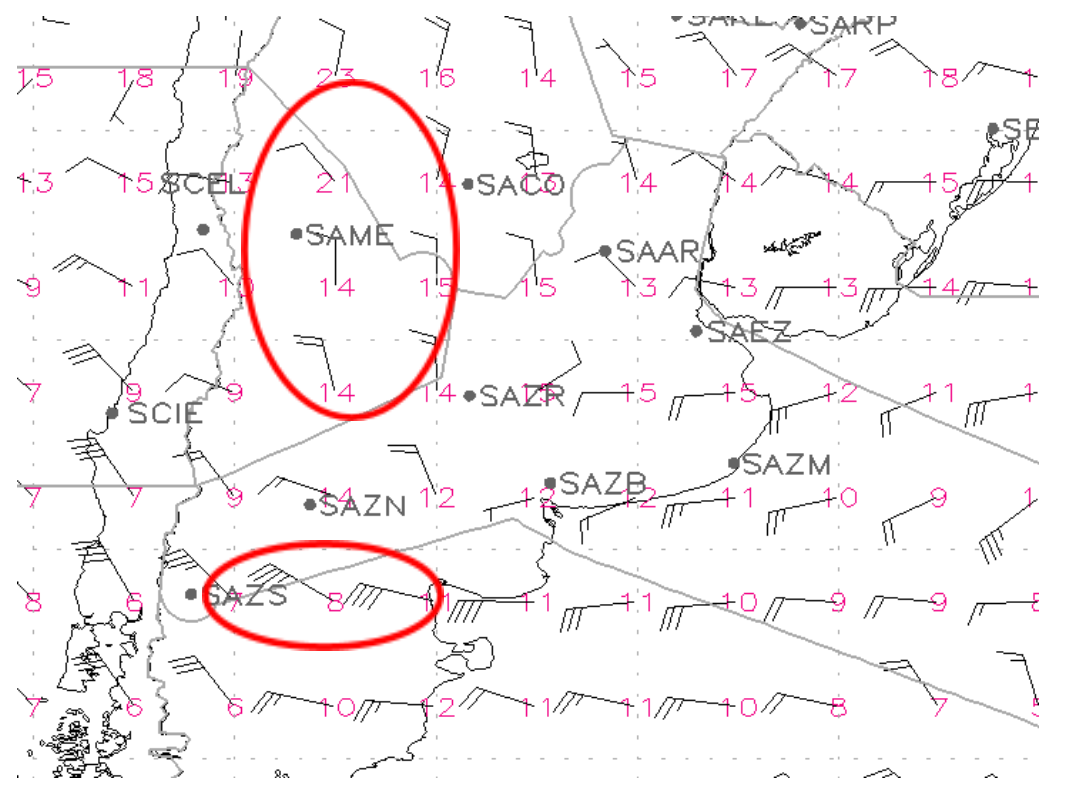
\includegraphics[width=0.85\linewidth]{Figuras/viento/mapaBarbas.png}
    \caption{Representación del viento en 850 \unit{\hecto\pascal} para el día 14/4/2016 a las 12 UTC en la región central de Argentina \cite{cursoObservadores2024}.}
    \label{fig:mapaBarbas}
\end{figure}

Las \textbf{líneas de corriente} \cite{recordAntarticos2024} son la representación gráfica más comúnmente utilizada para analizar los factores de la circulación a gran escala. Una línea de corriente se define como la curva cuya tangente en cualquiera de sus puntos coincide con la dirección de la velocidad del aire. Generalmente, se emplean en niveles altos y en superficie en zonas tropicales debido a su capacidad para ilustrar patrones de flujo de aire de manera clara y precisa. Un ejemplo de esta representación se puede observar en la Figura \ref{fig:mapaLineas}. En dicha figura, se muestra que un sistema de alta presión se desplazó hacia el sur de la Patagonia argentina. Este desplazamiento provocó el ingreso de aire templado a la península antártica, lo que a su vez generó condiciones de subsidencia. La subsidencia es el proceso mediante el cual el aire desciende en la atmósfera, aumentando su temperatura y reduciendo su humedad relativa. Este fenómeno intensificó el efecto de secado y calentamiento del aire al descender hacia la superficie, creando un ambiente más seco y cálido en la región.


\begin{figure}[H]
    \centering
    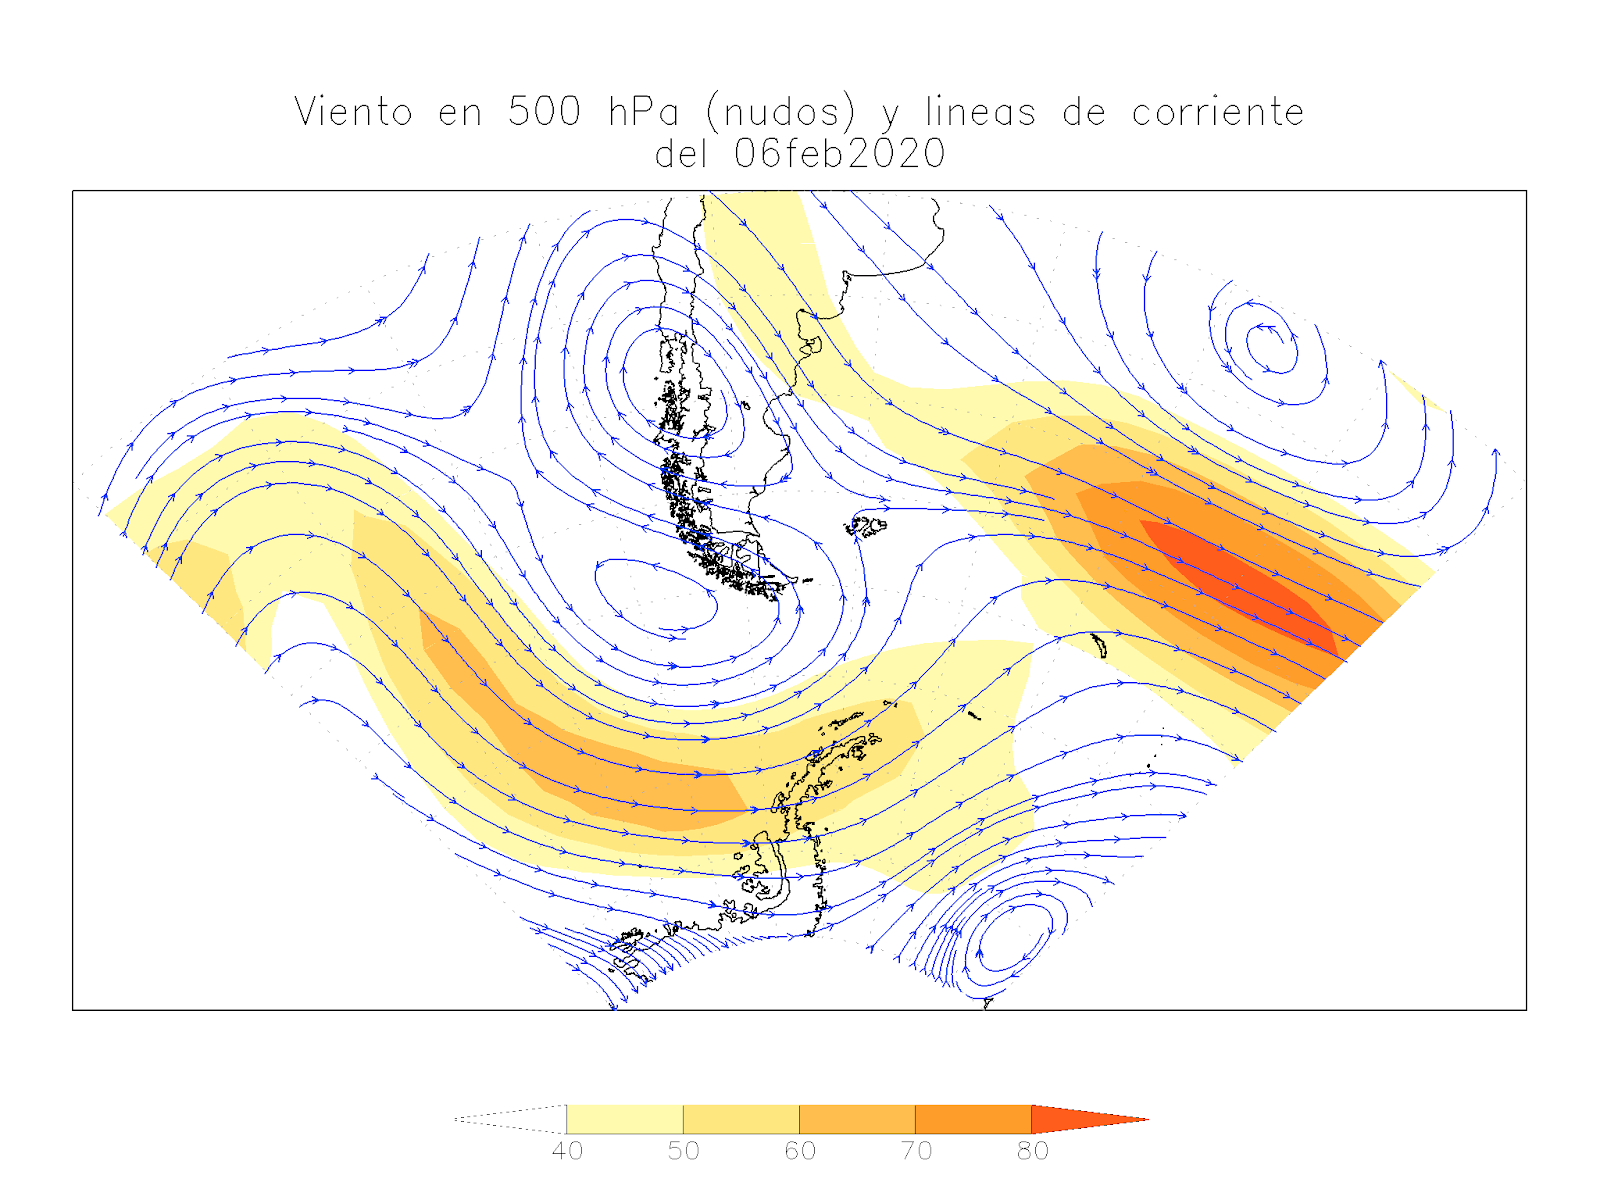
\includegraphics[width=1\linewidth]{Figuras/viento/mapalineasViento.png}
    \caption{Viento (nudos) y líneas de corriente en 500\unit{\hecto\pascal} \cite{recordAntarticos2024}.}
    \label{fig:mapaLineas}
\end{figure}


% Si fuera necesario hablar de las fuerzas que actúan sobre el movimiento del aire
%%%%%%%%%%%%%%%%%%%%%%%%%%%%%%%%%%%%%%%%%%%%%%%%%%%%%%%%%%%%%%%%%%%%%%%%%%%%%%%%%%%%%%%%%%%%%%%%%%%%%%%%%%%%%%%%%%%%%%%%
\section{Instrumentos de medición del viento}\label{sec:instrumentos_med_viento}
La medición precisa del viento en superficie requiere el uso de diversos instrumentos especializados, cada uno diseñado para capturar diferentes aspectos del flujo de aire. Estos instrumentos son esenciales para obtener datos confiables que se utilizan en múltiples aplicaciones meteorológicas y científicas. A continuación, se describen algunos de los instrumentos más comunes y su funcionamiento.

\subsection*{Sensor de Copas y Veleta}

En la Figura \ref{fig:copas_y_veleta} se muestra el sensor de copas y veleta, y es uno de los instrumentos más comunes para medir la velocidad y dirección del viento. Este dispositivo utiliza copas montadas en un eje vertical que giran con el viento, mientras que una veleta alineada con la dirección del viento proporciona datos direccionales. La velocidad de rotación de las copas se convierte en una medida de la velocidad del viento.
\begin{figure}[H]
    \centering
    \begin{minipage}[b]{0.4\textwidth}
        \centering
        \subcaptionbox{\label{fig:coperola}}{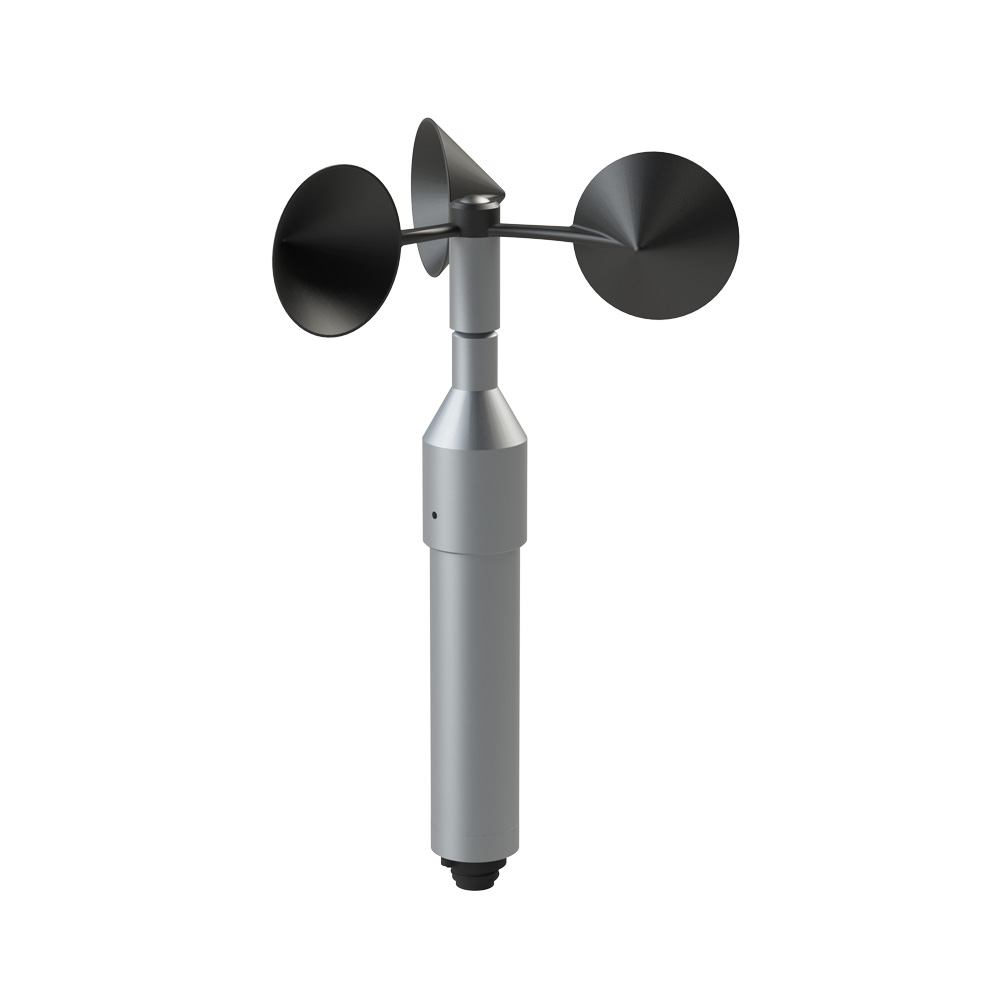
\includegraphics[width=\textwidth]{Figuras/viento/sensores/coperola.png}}
    \end{minipage}%
    \hspace{1em} % Espacio horizontal entre las columnas
    \begin{minipage}[b]{0.4\textwidth}
        \centering
        \subcaptionbox{\label{fig:veleta}}{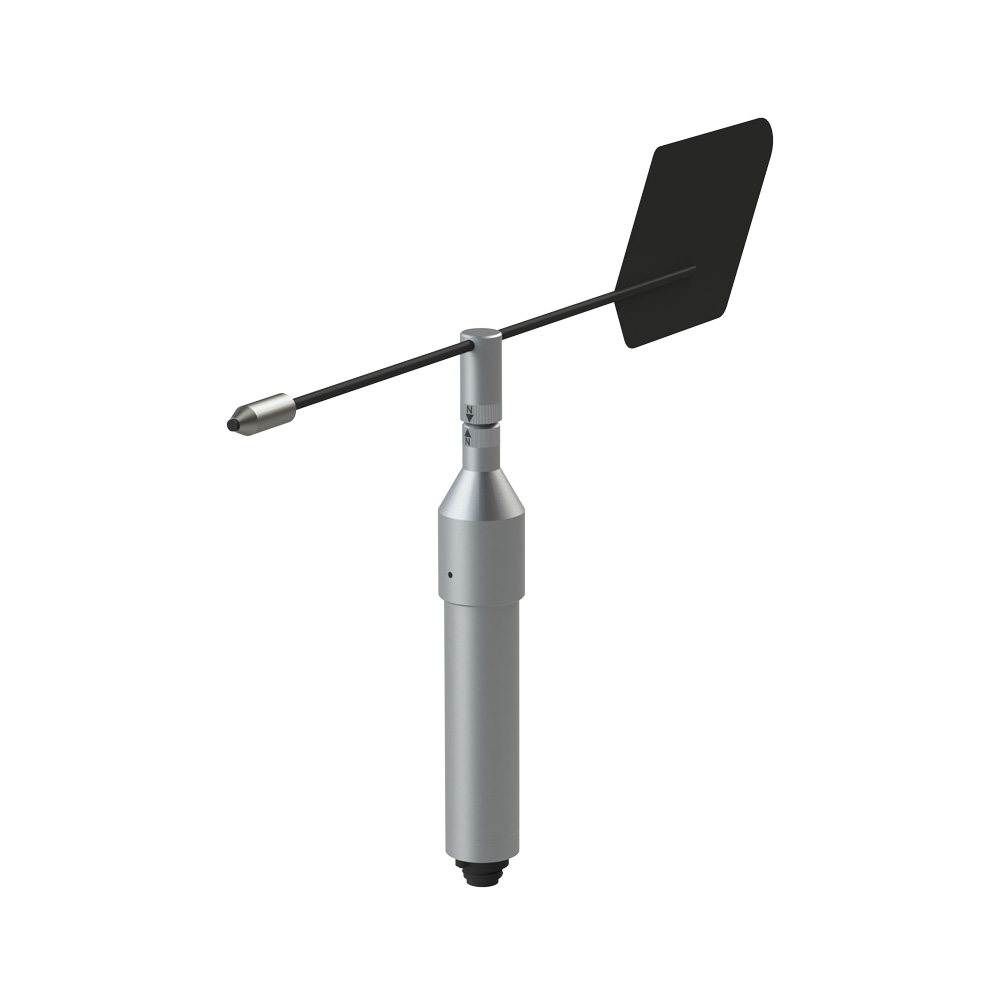
\includegraphics[width=\textwidth]{Figuras/viento/sensores/veleta.png}}
    \end{minipage}%
    \caption{En (a) el sensor de coperola y en (b) el sensor de veleta \cite{siapmicros2024}.}
    \label{fig:copas_y_veleta}
\end{figure}
\subsection*{Anemómetro de Hilo Caliente}

El anemómetro de hilo caliente que se muestra en la Figura \ref{fig:hiloCaliente} mide la velocidad del viento basándose en la tasa de enfriamiento de un hilo calentado eléctricamente. A medida que el viento pasa sobre el hilo, la tasa de enfriamiento varía con la velocidad del viento, permitiendo así su medición. Este tipo de anemómetro es especialmente útil para medir velocidades de viento bajas y en estudios de flujo de aire en túneles de viento.

\begin{figure}[H]
    \centering
    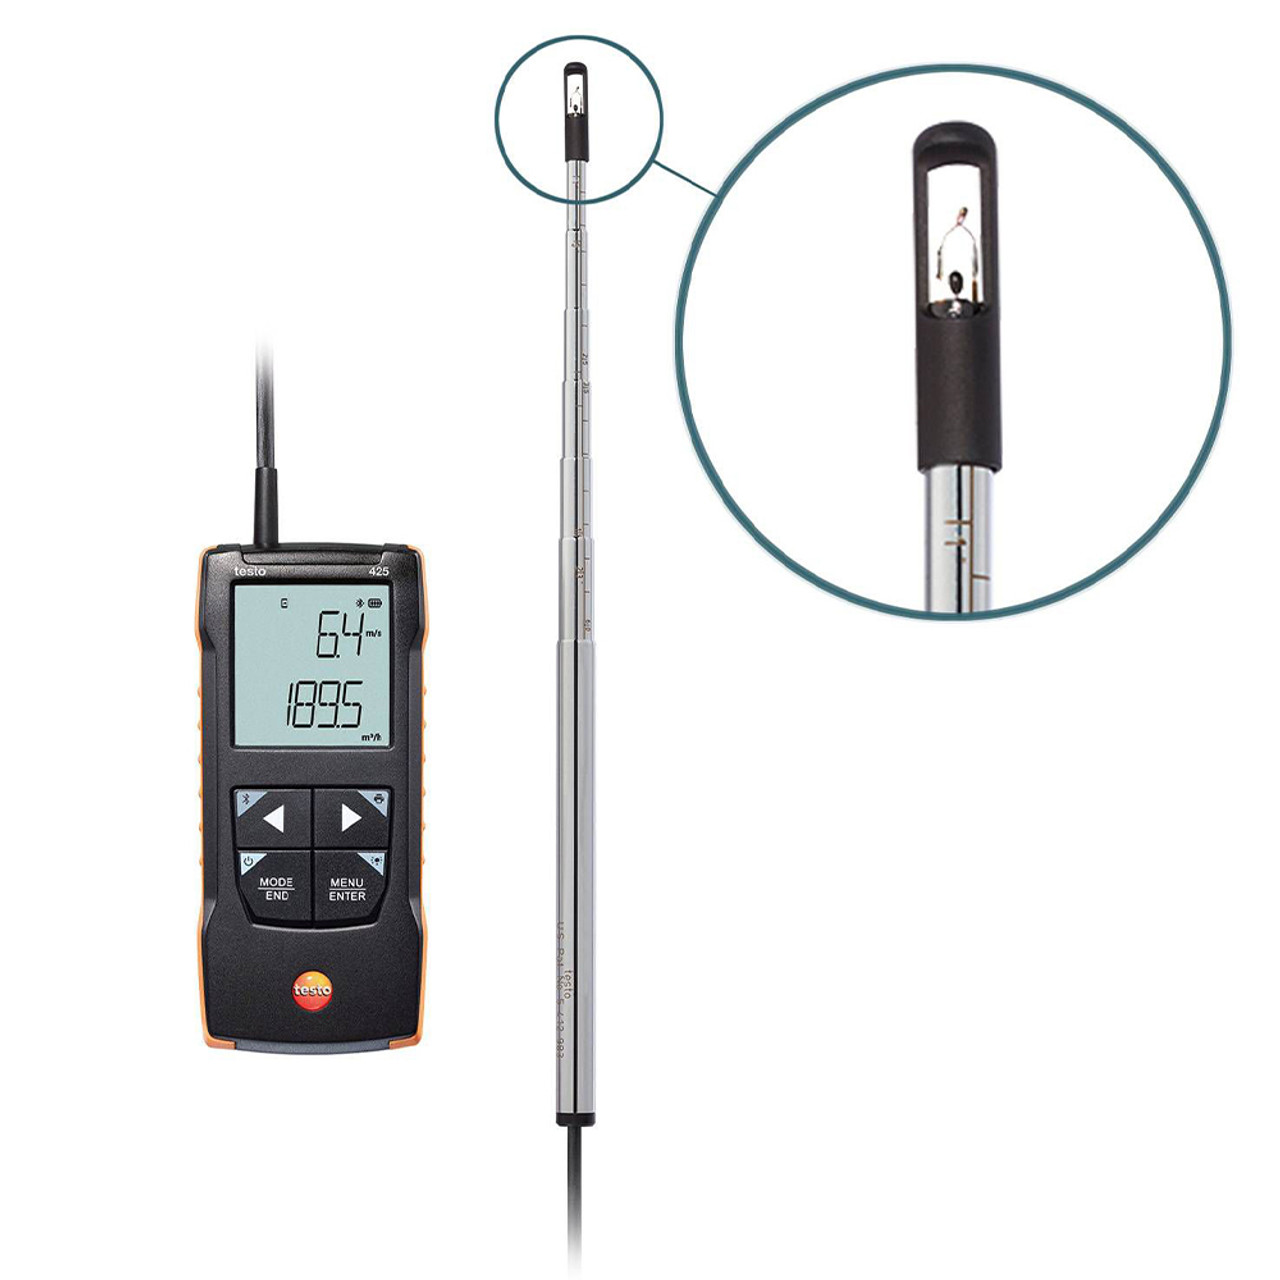
\includegraphics[width=0.5\textwidth]{Figuras/viento/sensores/hiloCaliente.png}
    \caption{Anemómetro de hilo caliente \cite{testoAnemometer}.}
    \label{fig:hiloCaliente}
\end{figure}

\subsection*{Tubo Pitot}

El tubo Pitot  de la Figura \ref{fig:tuboPitot}, mide la velocidad del viento a través de la diferencia de presión entre un tubo orientado contra el flujo de aire y un tubo estático. Esta diferencia de presión se convierte en una medida de la velocidad del viento. Los tubos Pitot son ampliamente utilizados en aplicaciones aeronáuticas y en estudios de dinámica de fluidos.

\begin{figure}[h]
    \centering
    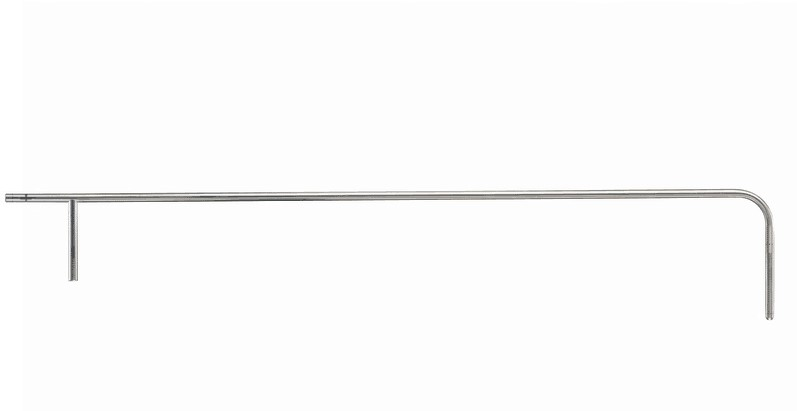
\includegraphics[width=0.7\textwidth]{Figuras/viento/sensores/tuboPitot.jpg}
    \caption{Tubo Pitot \cite{testoAnemometer}.}
    \label{fig:tuboPitot}
\end{figure}

\subsection*{Anemómetro de Ultrasonido}

El anemómetro de ultrasonido con el cual trabajaremos en esta tesis es similar al de la Figura \ref{fig:ultrasonido}, en general estos sensores utilizan ondas sonoras para medir la velocidad y dirección del viento. Emite pulsos ultrasónicos entre transductores y mide el tiempo que tardan en viajar entre ellos. La diferencia en el tiempo de viaje se utiliza para calcular la velocidad del viento. Este tipo de anemómetro es preciso y no tiene partes móviles, lo que reduce el mantenimiento. Se da una explicación mas detallada de su funcionamiento en el apéndice \ref{ap:principioDeMedicionUltrasonido}.

\begin{figure}[h]
    \centering
    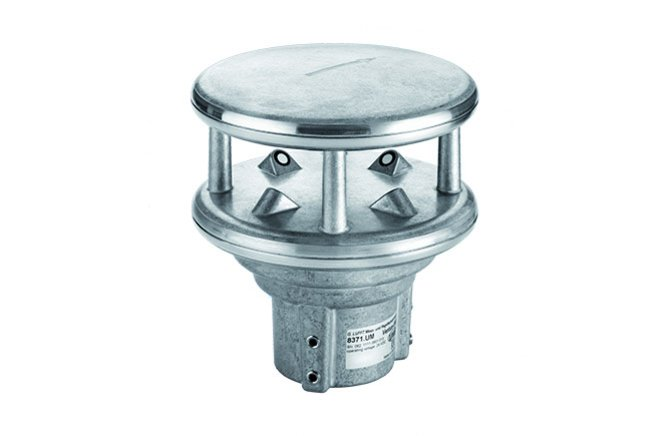
\includegraphics[width=0.6\textwidth]{Figuras/viento/sensores/ultrasonido.png}
    \caption{Anemómetro de ultrasonido \cite{ventusumb2024}.}
    \label{fig:ultrasonido}
\end{figure}

\subsection*{Anemómetro Láser Doppler}

El anemómetro láser Doppler mide la velocidad del viento utilizando el efecto Doppler de la luz láser. Como se ve en la Figura \ref{fig:laserDoppler}, un haz láser se dirige hacia partículas en el aire, y la luz dispersada se analiza para determinar el cambio en la frecuencia debido al movimiento de las partículas. Este cambio se convierte en una medida de la velocidad del viento. Este tipo de anemómetro es altamente preciso y se utiliza en investigaciones avanzadas de dinámica de fluidos.

\begin{figure}[h]
    \centering
    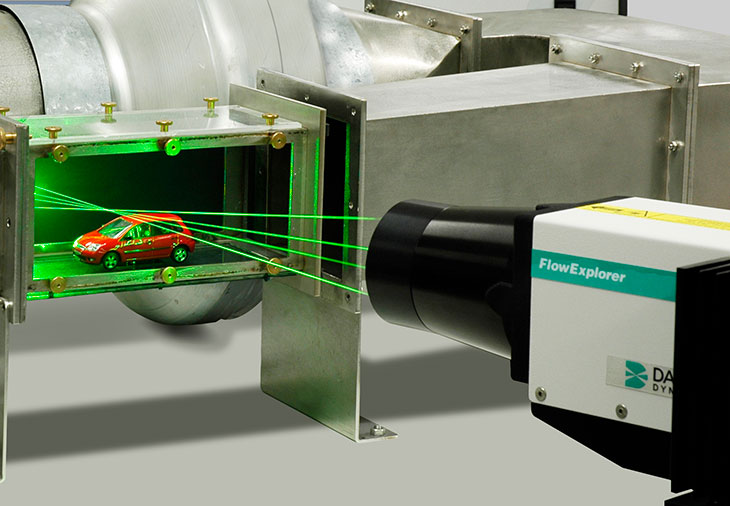
\includegraphics[width=0.7\textwidth]{Figuras/viento/sensores/laserDoppler.png}
    \caption{Anemómetro láser Doppler \cite{dantecLDA2024}.}
    \label{fig:laserDoppler}
\end{figure}


% Aca dar el detalle de los manuales de Vaisala y DeltaOHM, como se mide el viento, sus partes y como se debe alinear en la instalacion, sacar todo de los manuales, mencionar por arriba la coperola, el anemo de hilo caliente y el laserdoplerlidar.


%%%%%%%%%%%%%%%%%%%%%%%%%%%%%%%%%%%%%%%%%%%%%%%%%%%%%%%%%%%%%%%%%%%%%%%%%%%%%%%%%%%%%%%%%%%%%%%%%%%%%%%%%%%%%%%%%%%%%%%%
\section{Túnel de viento}\label{tunelDeViento}

El Servicio Meteorológico Nacional (SMN) cuenta con un túnel de viento con una antigüedad de aproximadamente 50 años, fabricado por la empresa \textit{Santos Zaghi}. Este túnel se utiliza para la verificación de distintos tipos de anemómetros, detallados en la sección \ref{sec:instrumentos_med_viento}. El rango de velocidad del viento que actualmente alcanza está entre \SI{1}{\meter\per\second} y \SI{26}{\meter\per\second}, lo cual es adecuado para los anemómetros instalados en el campo de observación. En la Figura \ref{fig:tunelVientoEsquema} se muestra un esquema donde se observan las partes que lo componen: el motor que gira una hélice, el variador con su tablero de control y la zona de medición donde se instalan el sensor de viento bajo prueba y el patrón de referencia, en particular, de la marca Vaisala, modelo WMT700, con un rango de operación de \SI{0.01}{\meter\per\second} a \SI{65}{\meter\per\second} y una resolución de \SI{0.01}{\meter\per\second}. El sistema de referencia utilizado es el que se indica en la figura, donde la altura se mide en el eje vertical, la profundidad en el eje transversal y la longitud en el eje longitudinal.

\begin{figure}[H]
    \centering
    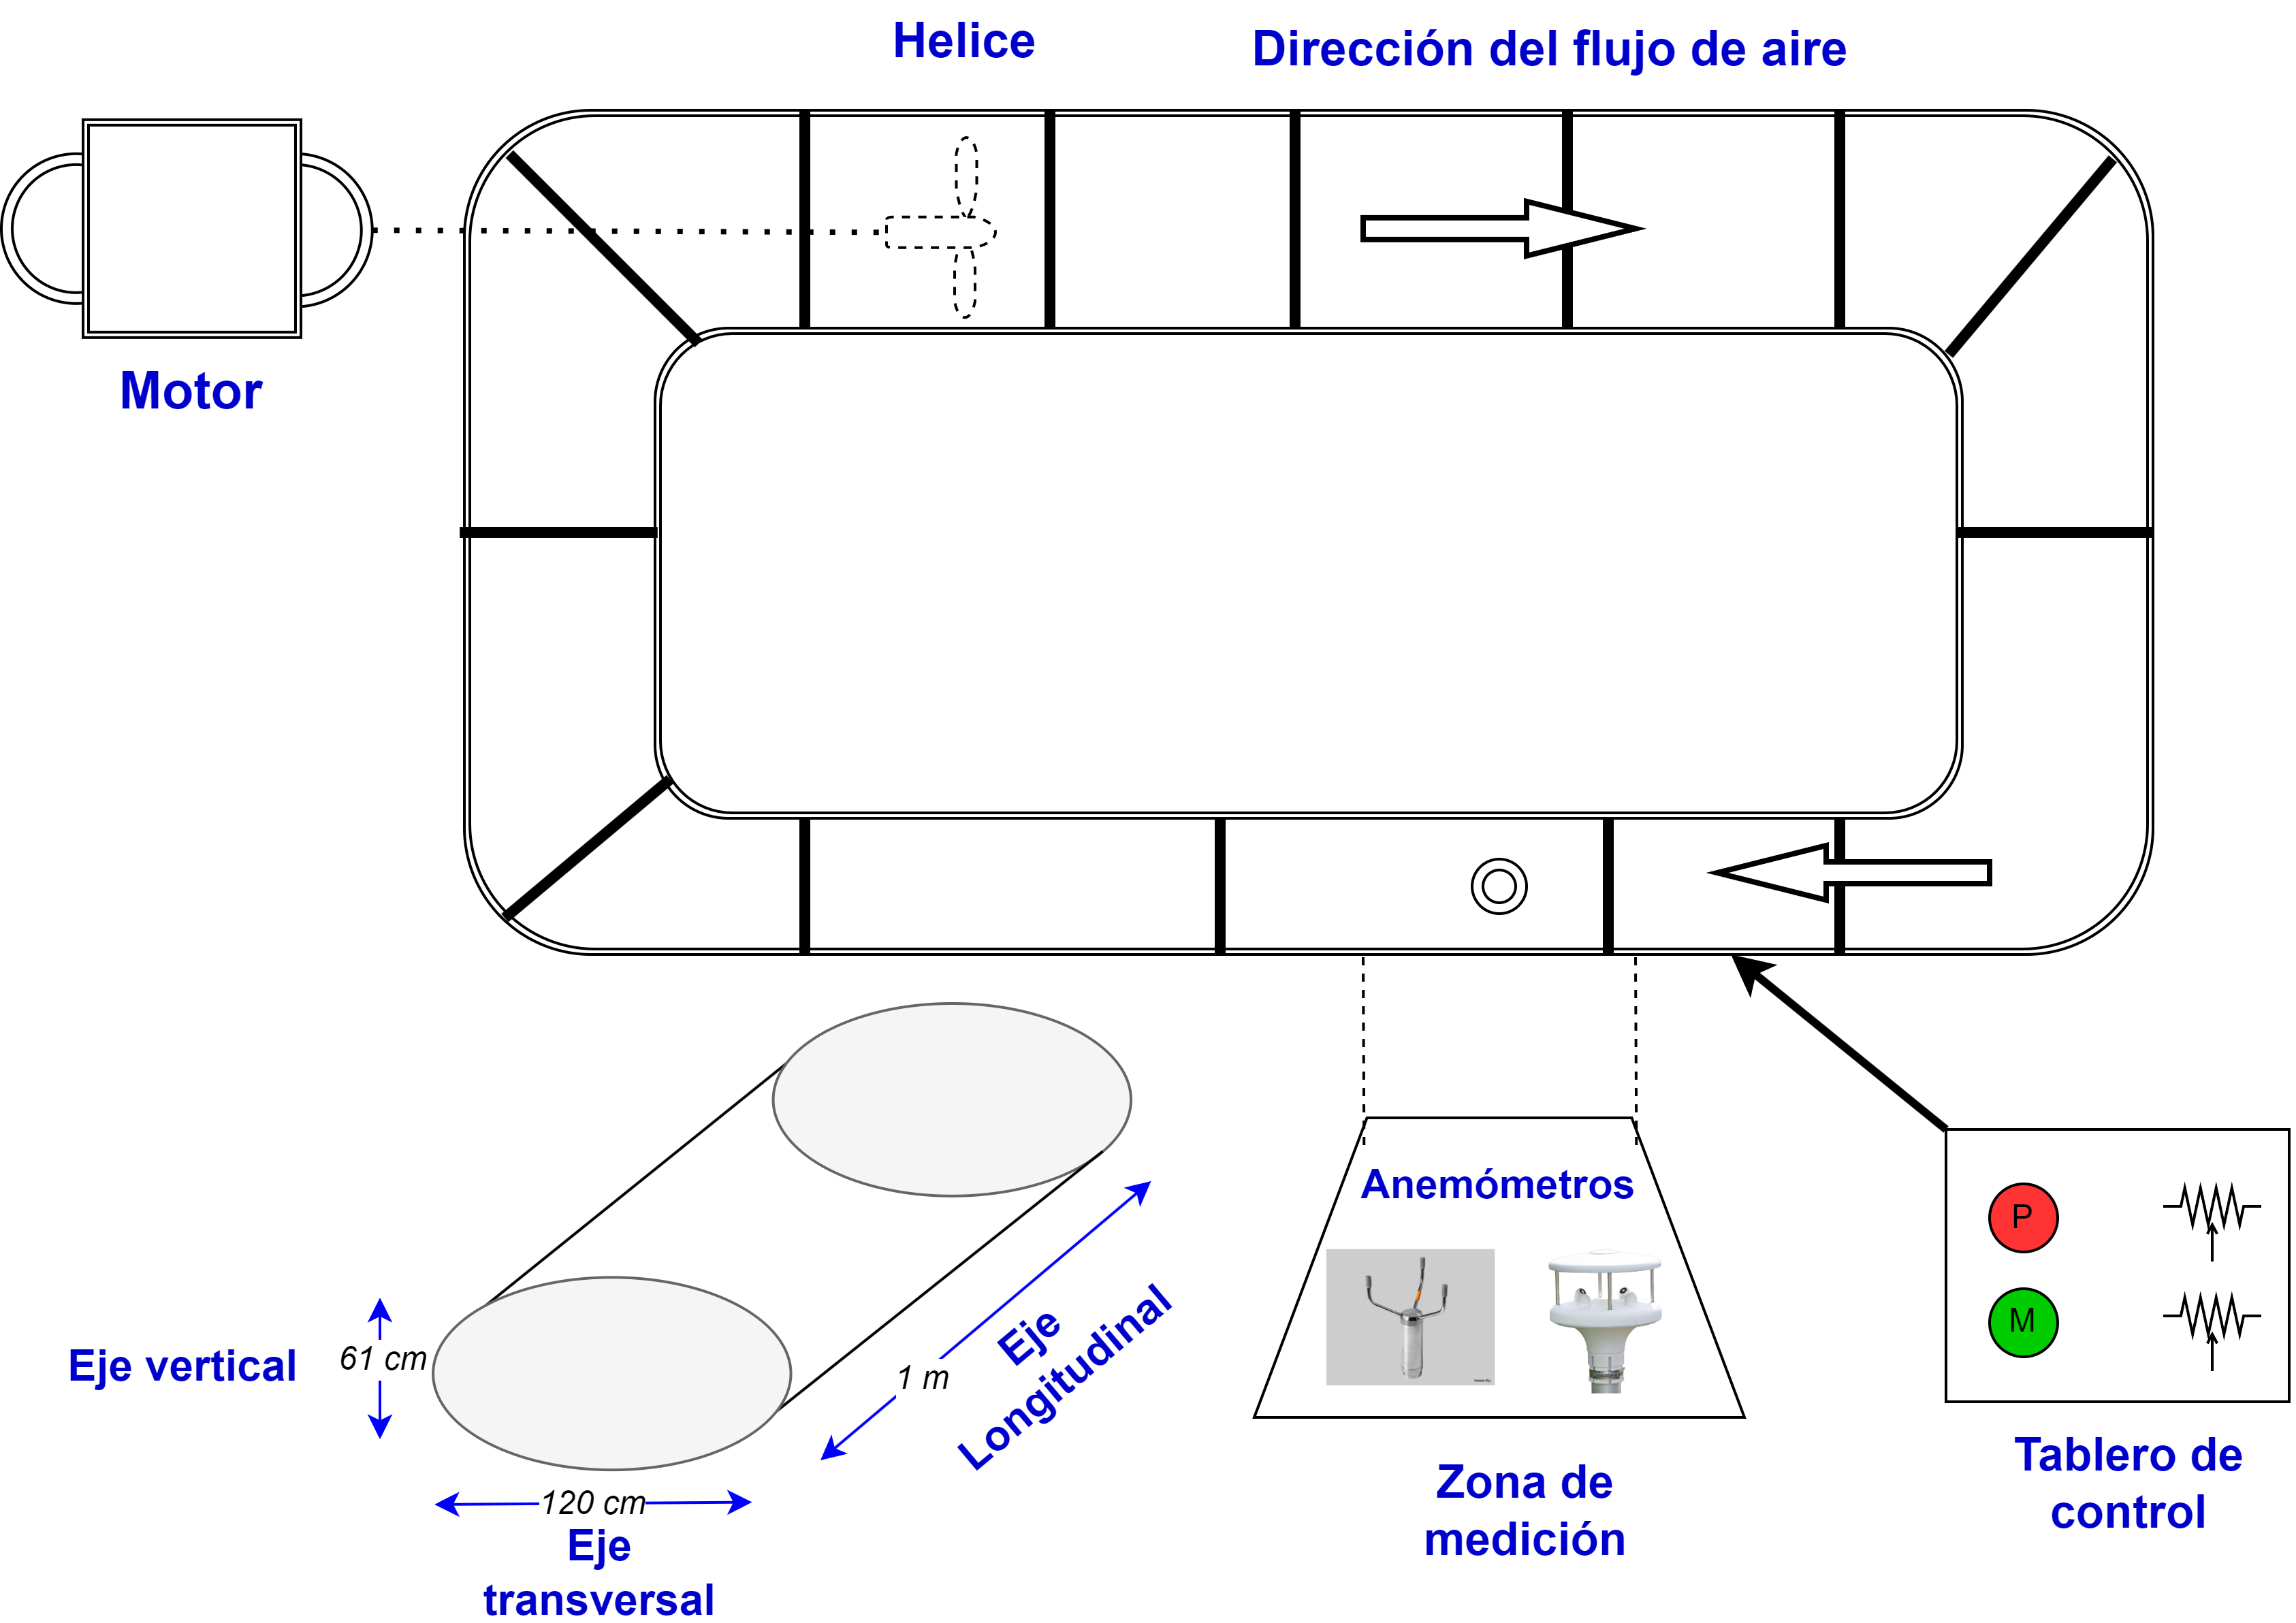
\includegraphics[width=0.9\linewidth]{Figuras/viento/tunelDeViento/TunelVientoEsquema.png}
    \caption{Esquema del túnel de viento.}
    \label{fig:tunelVientoEsquema}
\end{figure}

En la Figura \ref{fig:tuneDeViento2} se muestra una foto del túnel de viento, es de tipo cerrado con un perímetro medio de $\SI{21}{\meter}$. A la izquierda, en la parte inferior se encuentra el motor.

\begin{figure}[H]
    \centering
    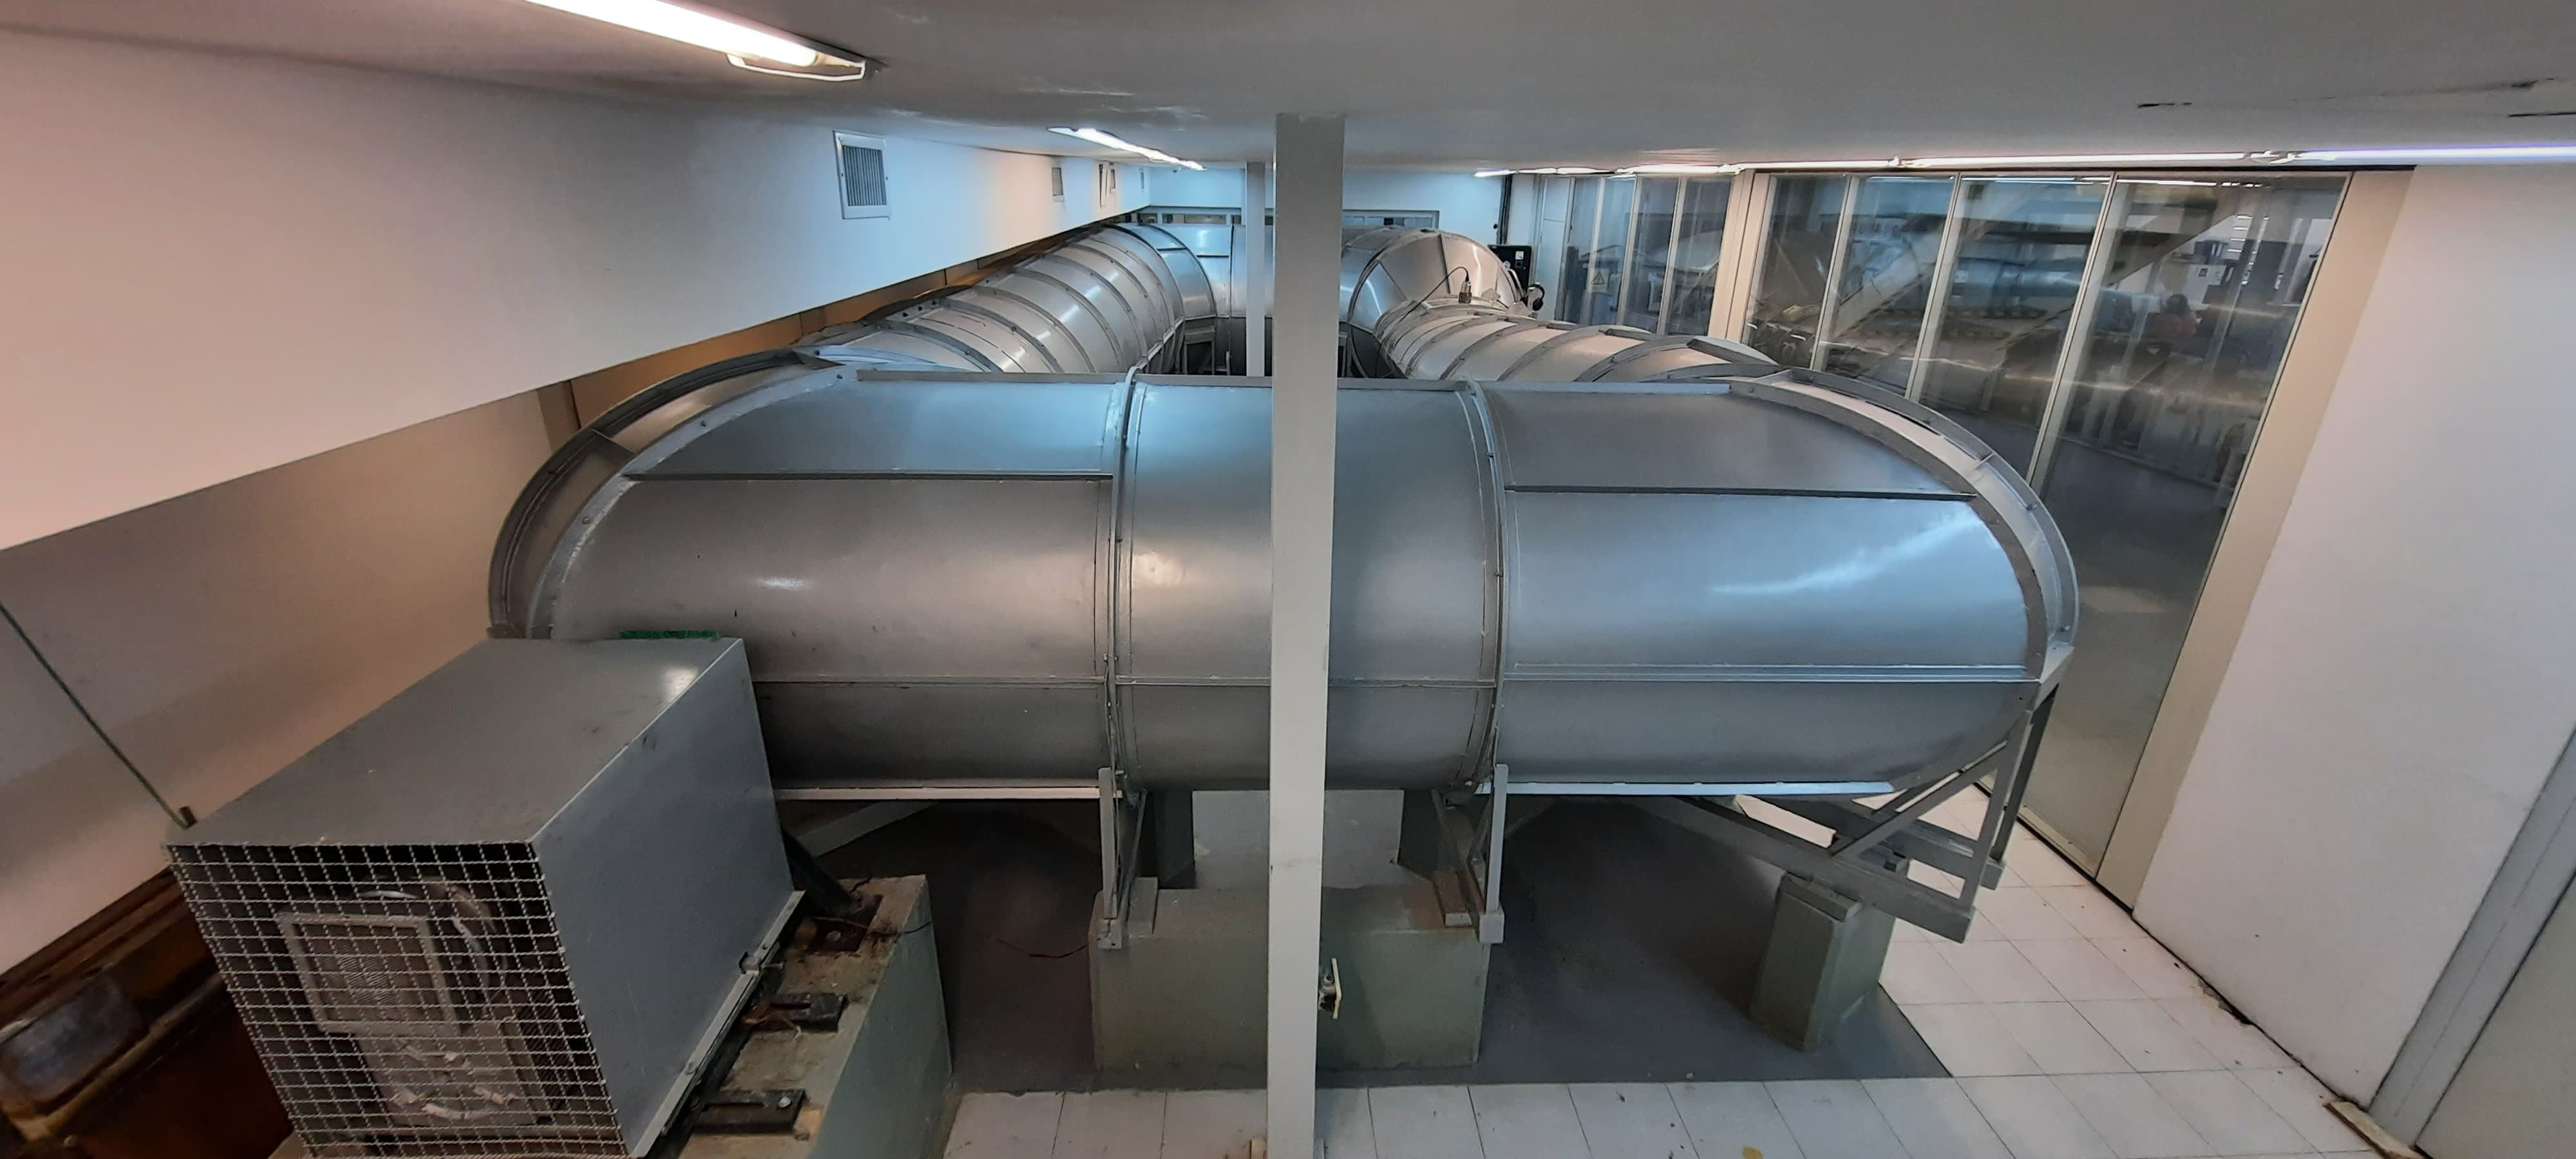
\includegraphics[width=0.9\linewidth]{Figuras/viento/tunelDeViento/tuneDeViento2.jpg}
    \caption{Vista general del túnel de viento cerrado del SMN.}
    \label{fig:tuneDeViento2}
\end{figure}

En la Figura \ref{fig:zonaMedicionTapaCerrada} se muestra la parte externa de la zona de medición, la cual tiene una longitud de $\SI{1}{\meter}$ en la dirección longitudinal. Como se observa en la Figura \ref{fig:zonaMedicionTapaAbierta}, en el centro hay una tapa con dimensiones de $\SI{33}{\centi\meter} \times \SI{28}{\centi\meter}$, que se abre para permitir el ingreso de los instrumentos y sus respectivos soportes. En la Figura \ref{fig:soporteParaBrazoConAnemos}, se muestra una barra cilíndrica telescópica\footnote{La altura es ajustable en el eje vertical.} montada en el suelo, la cual puede variar su altura hasta ingresar por un orificio en la parte baja del túnel, esta se utiliza para apoyar los sensores en un soporte.

\begin{figure}[H]
    \centering
    \begin{minipage}[b]{0.6\textwidth}
        \centering
        \subcaptionbox{\label{fig:zonaMedicionTapaCerrada}}{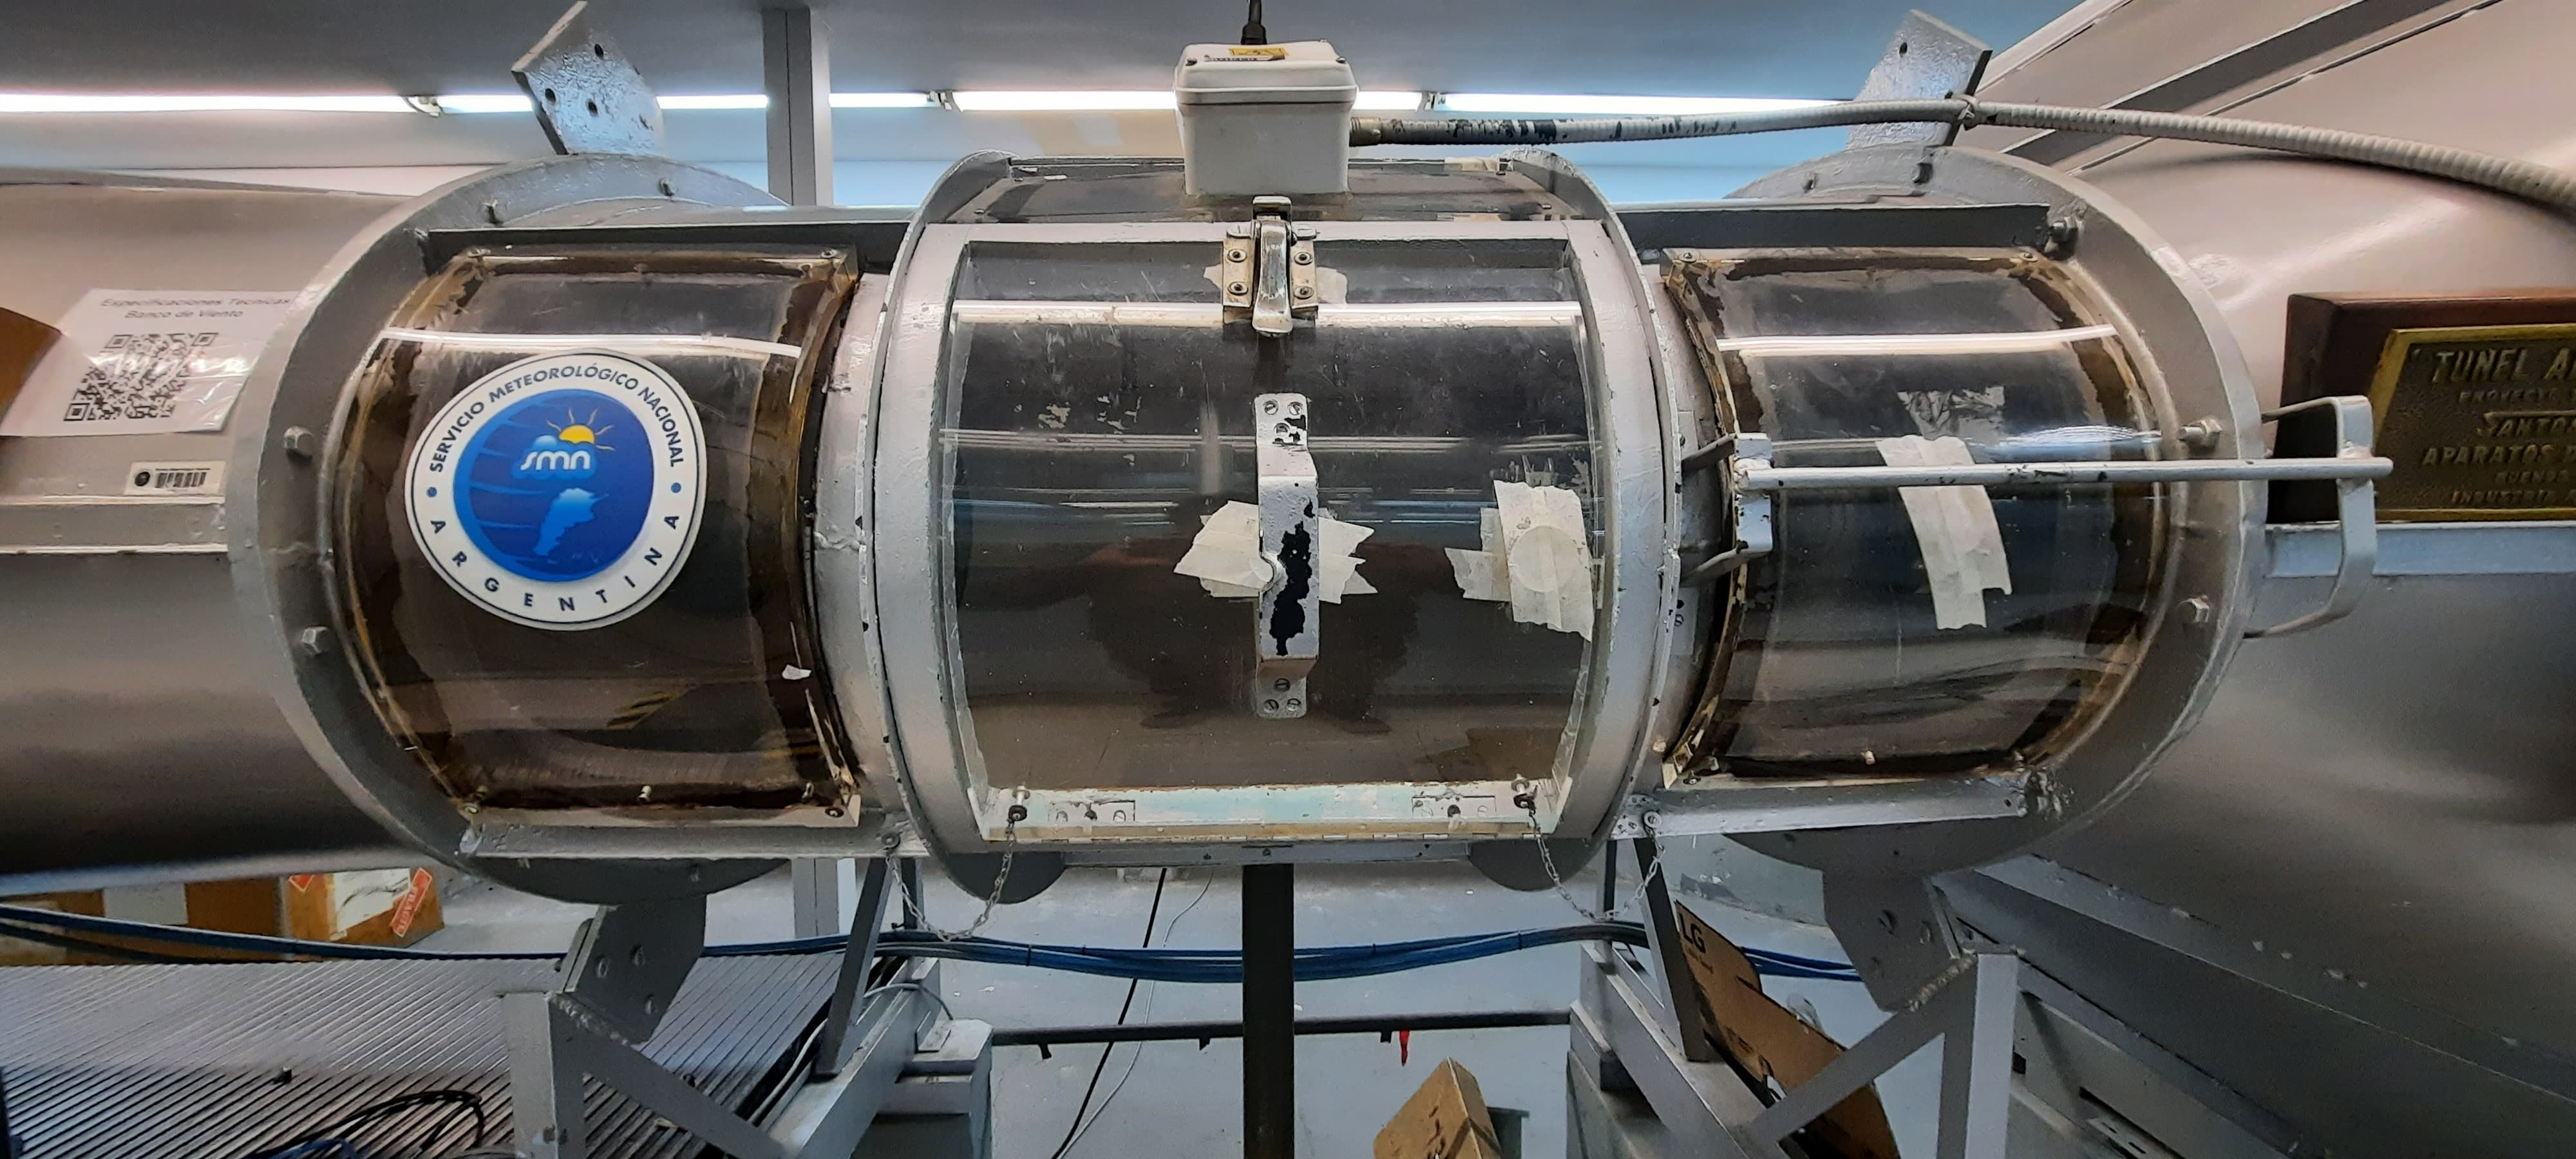
\includegraphics[width=\textwidth]{Figuras/viento/tunelDeViento/zonaMedicionTapaCerrada.jpg}}
        % \vspace{2em} % Espacio vertical entre las filas
        \subcaptionbox{\label{fig:zonaMedicionTapaAbierta}}{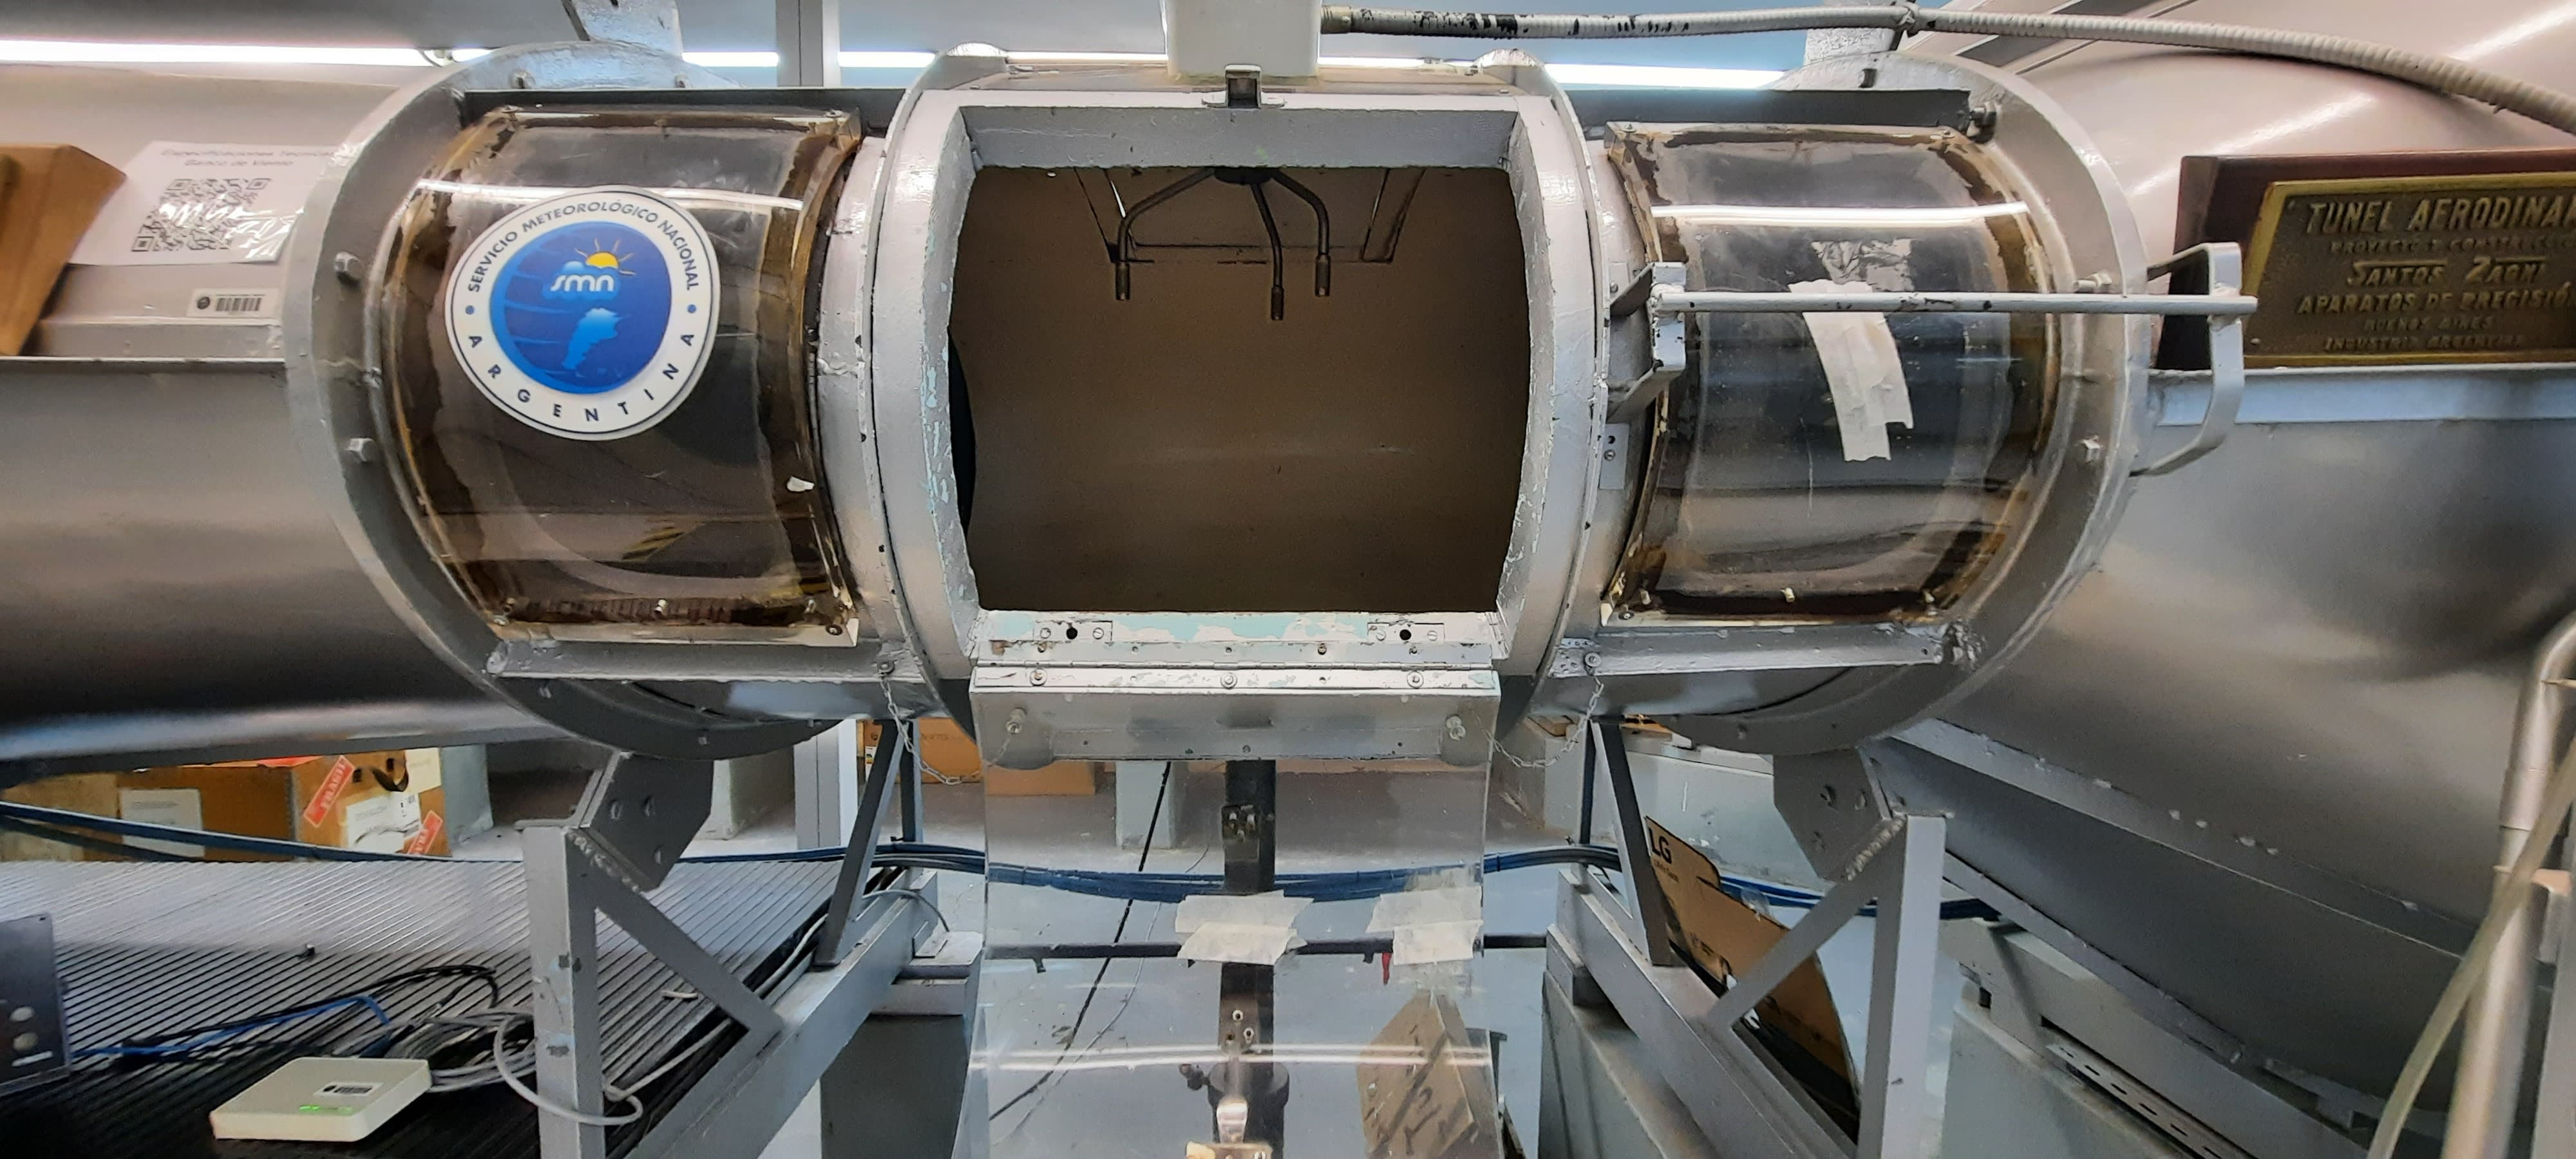
\includegraphics[width=\textwidth]{Figuras/viento/tunelDeViento/zonaMedicionTapaAbierta.jpg}}
    \end{minipage}%
    \hspace{1em} % Espacio horizontal entre las columnas
    \begin{minipage}[b]{0.35\textwidth}
        \centering
        \subcaptionbox{\label{fig:soporteParaBrazoConAnemos}}{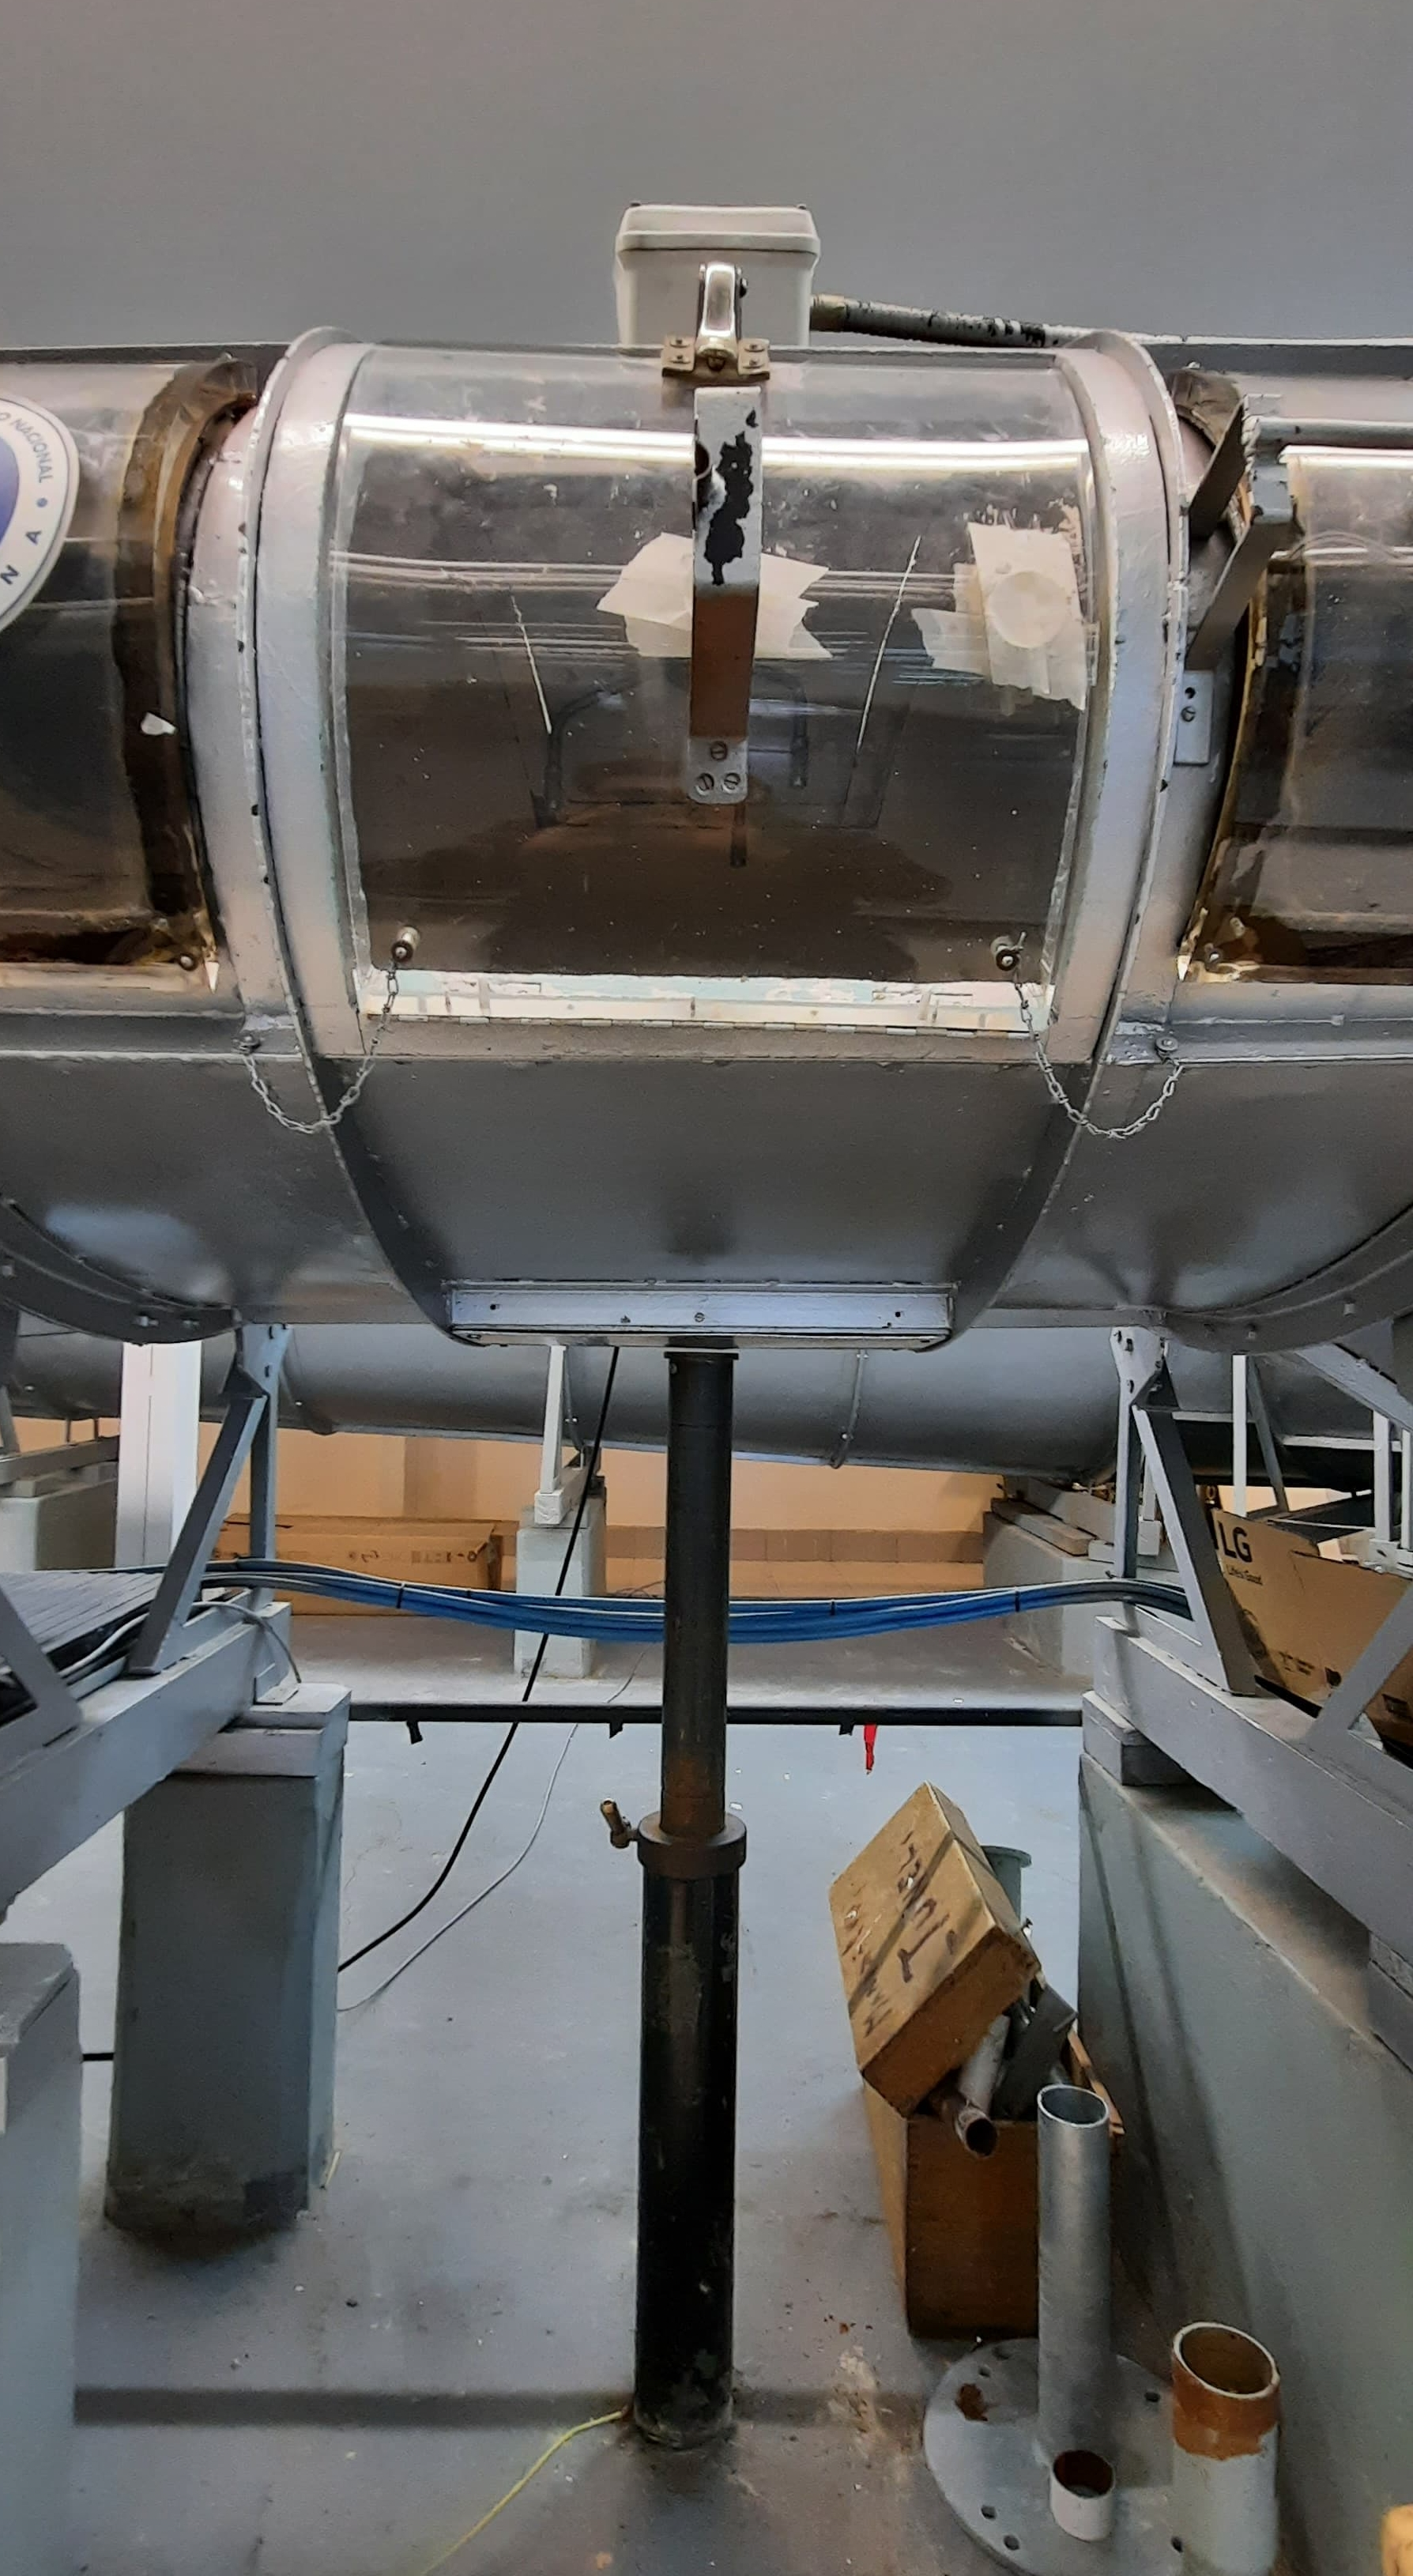
\includegraphics[width=\textwidth]{Figuras/viento/tunelDeViento/soporteParaBrazoConAnemos.jpg}}
    \end{minipage}
    
    \caption{En (a) se muestra la puerta cerrada de la zona de medición, en (b) se muestra la puerta abierta y en (c) se muestra la varilla telescópica.}
    \label{fig:tunelExterno}
\end{figure}

En la Figura \ref{fig:alabesIzquieda} se muestra el interior de la zona de medición, cuya sección transversal elíptica se diseñó para disminuir la turbulencia en las paredes y mejorar la homogeneidad del flujo de aire. Por otro lado, en la Figura \ref{fig:alabesDerecha} se observan los álabes (aleta de dirección), dispositivos esenciales que enderezan el flujo de aire, eliminando la componente rotacional inducida por el ventilador cuando atraviesa una esquina o cambio de sección abrupto. Esto no solo reduce la turbulencia, sino que también crea un flujo más uniforme y laminar, lo cual es crucial para obtener mediciones precisas y reproducibles en los ensayos aerodinámicos. 

En la Figura \ref{fig:zonaDeMedicion} se observa la zona de medición de \SI{1}{\meter} de largo, \SI{120}{\centi\meter} de ancho y \SI{61}{\centi\meter} de alto. Tanto el soporte como los anemómetros patrón y bajo calibración deben ser ubicados en esta zona, detallando la posición exacta en el volumen, para así lograr la reproducibilidad de las mediciones. Más adelante, en la sección \ref{sec:caracterZonaMed}, se mostrará un ensayo para caracterizar y encontrar dos posiciones tanto para el instrumento patrón, como para el instrumento bajo calibración.

\begin{figure}[H]
    \centering
    
    \begin{minipage}[b]{0.45\textwidth}
        % \centering
        \subcaptionbox{\label{fig:alabesIzquieda}}{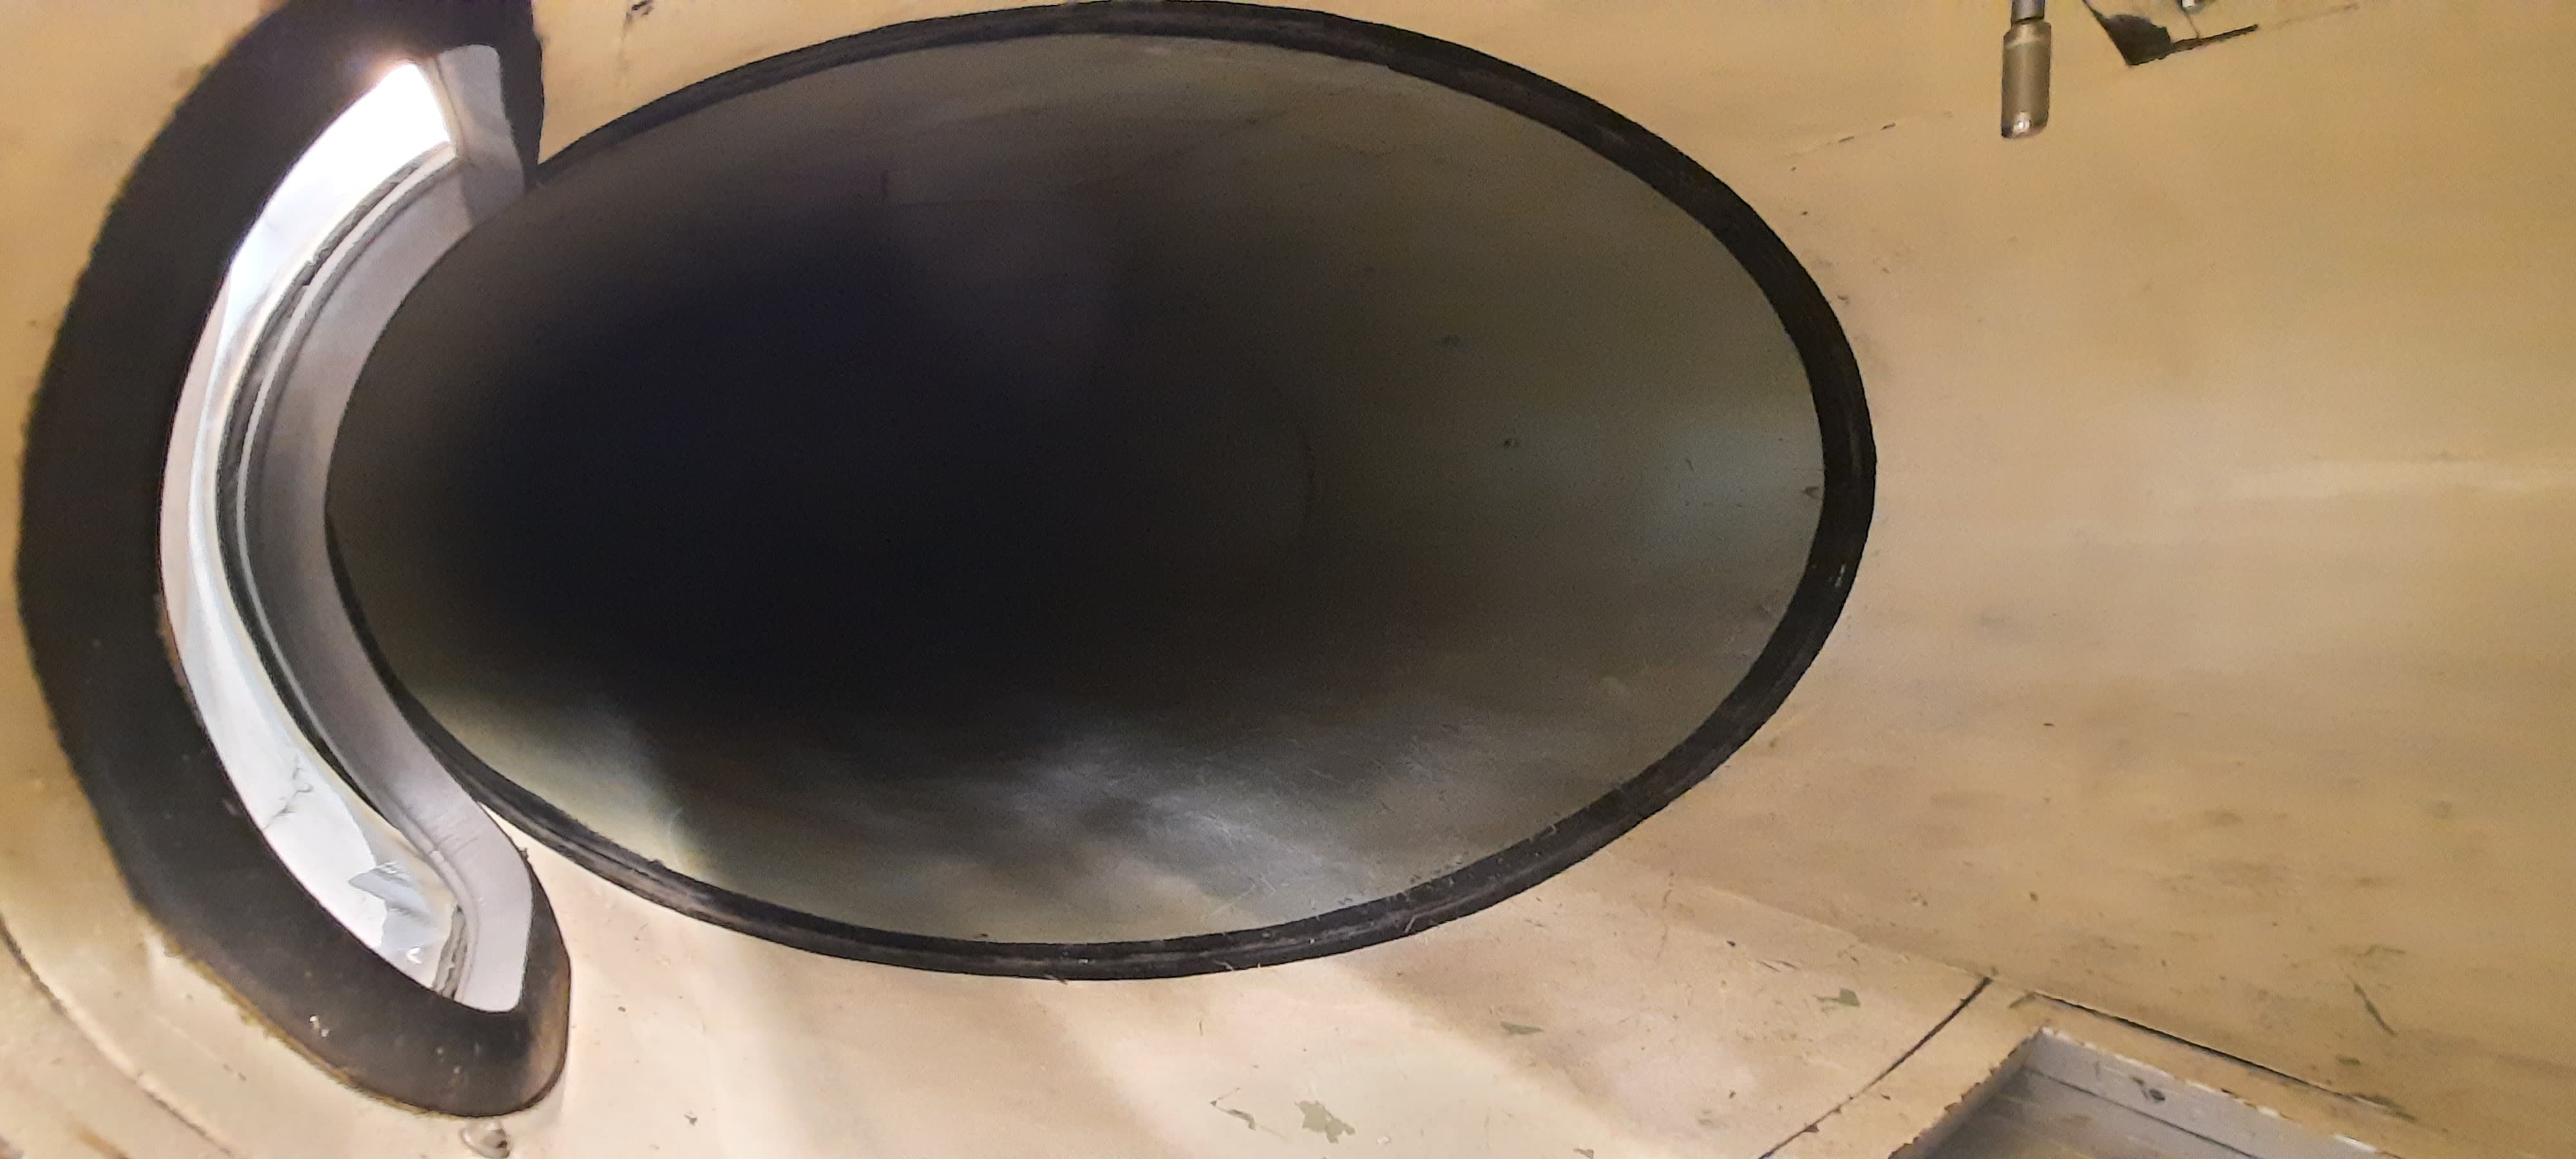
\includegraphics[width=\textwidth]{Figuras/viento/tunelDeViento/alabesIzquieda.jpg}}
    \end{minipage}
    \hspace{1em} % Espacio vertical entre las filas
    \begin{minipage}[b]{0.45\textwidth}
        \subcaptionbox{\label{fig:alabesDerecha}}{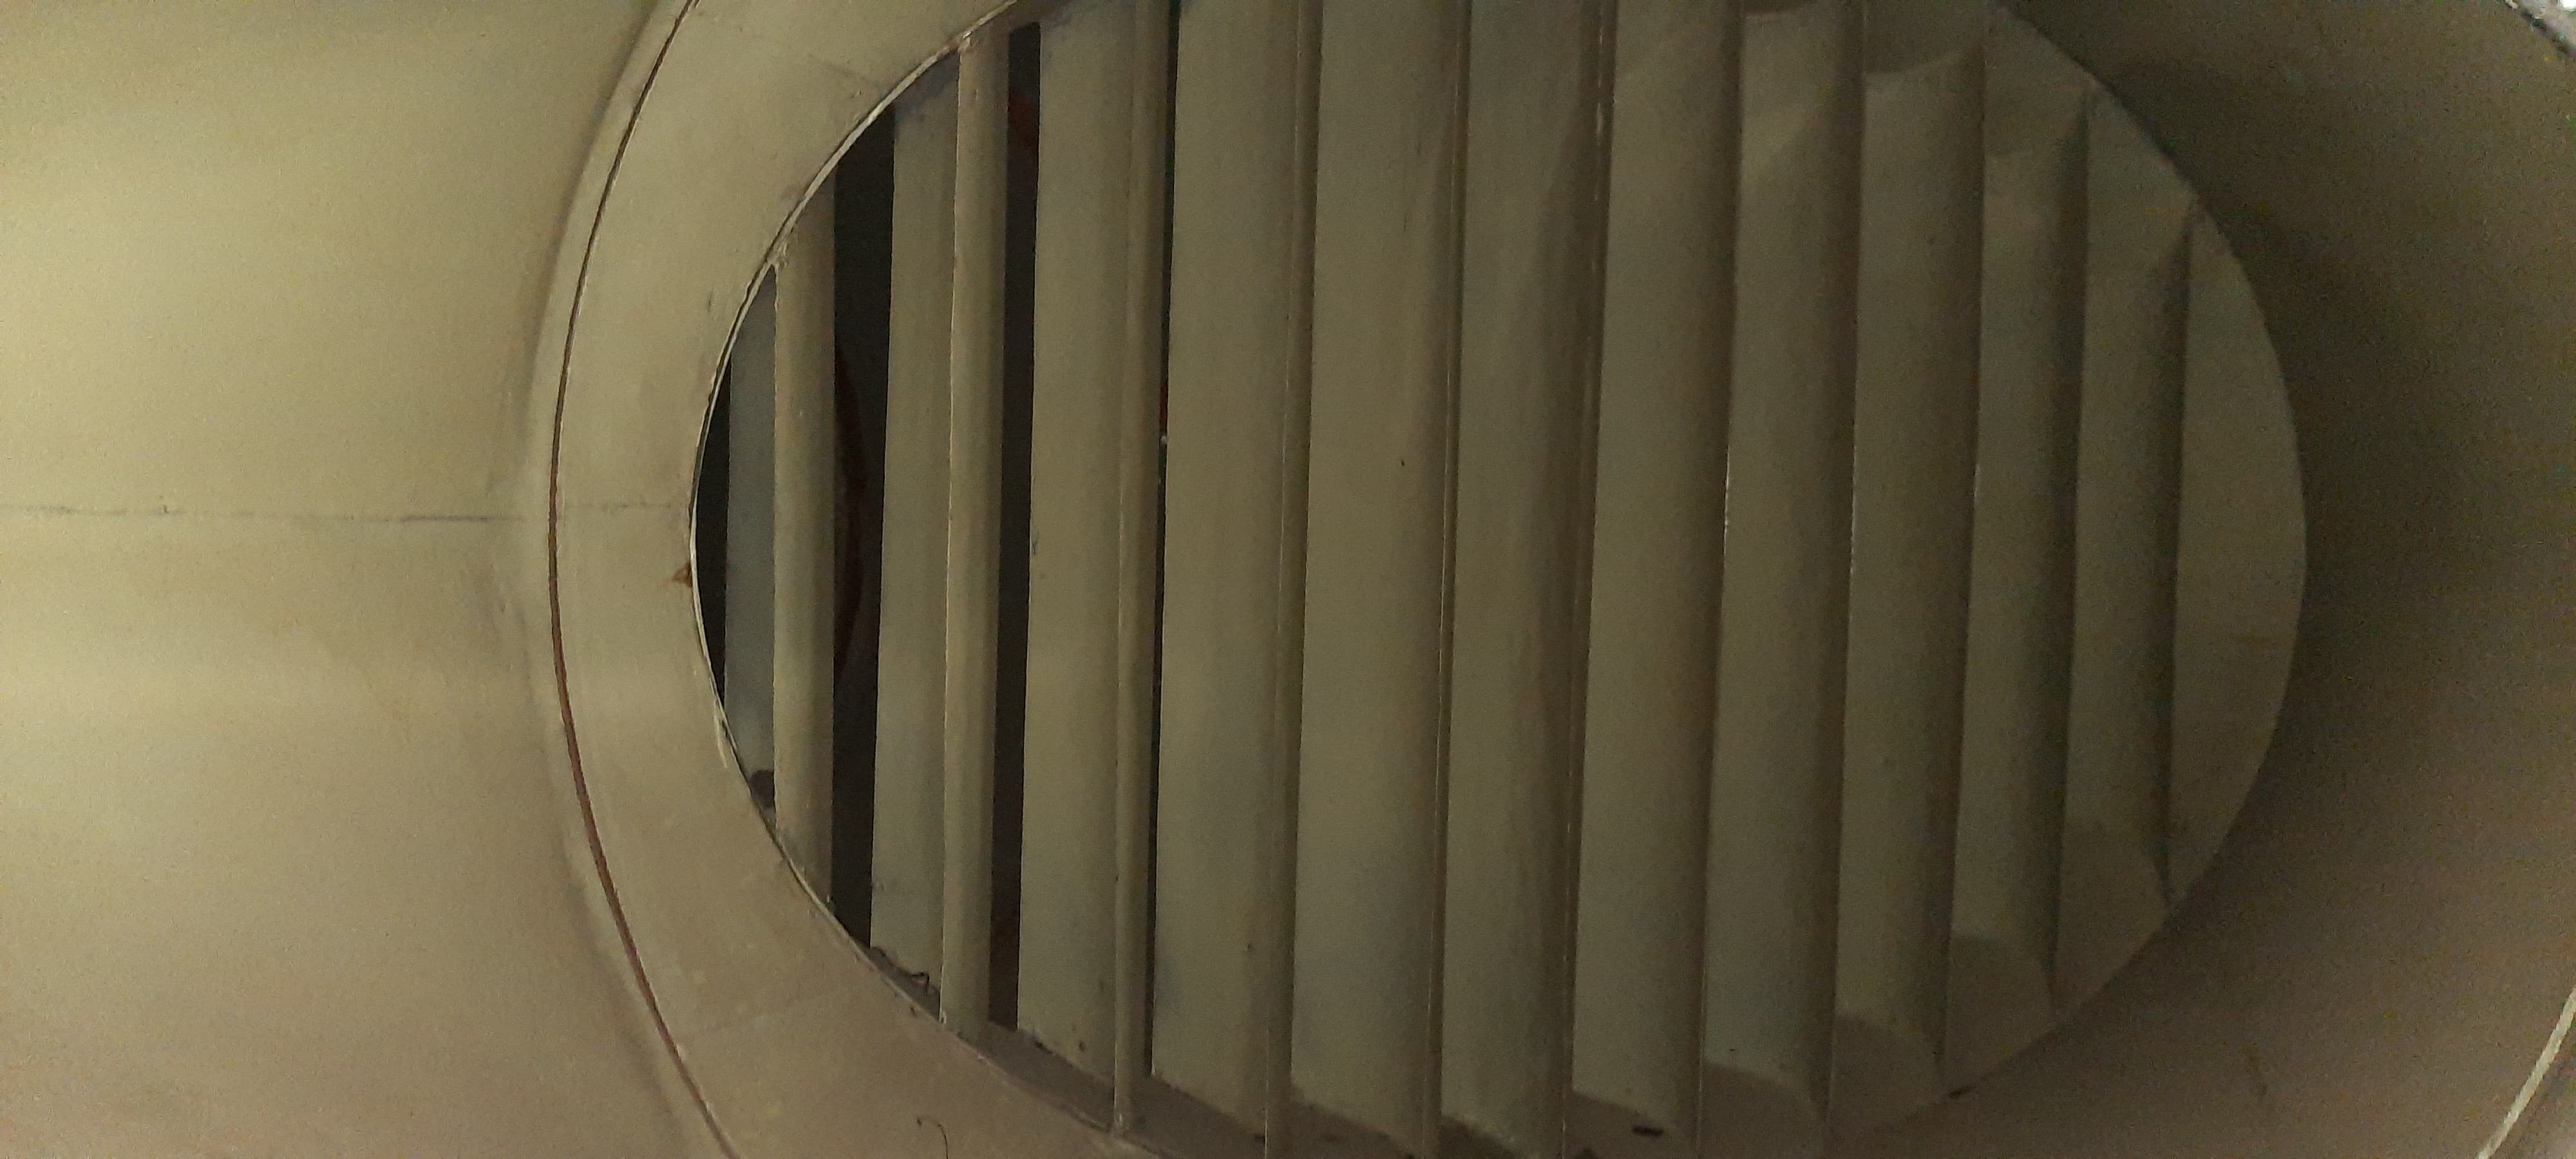
\includegraphics[width=\textwidth]{Figuras/viento/tunelDeViento/alabesDerecha.jpg}}
    \end{minipage}
    \vspace{1em} 
    \begin{minipage}{0.7\textwidth}
        \centering
        \subcaptionbox{\label{fig:zonaDeMedicion}}{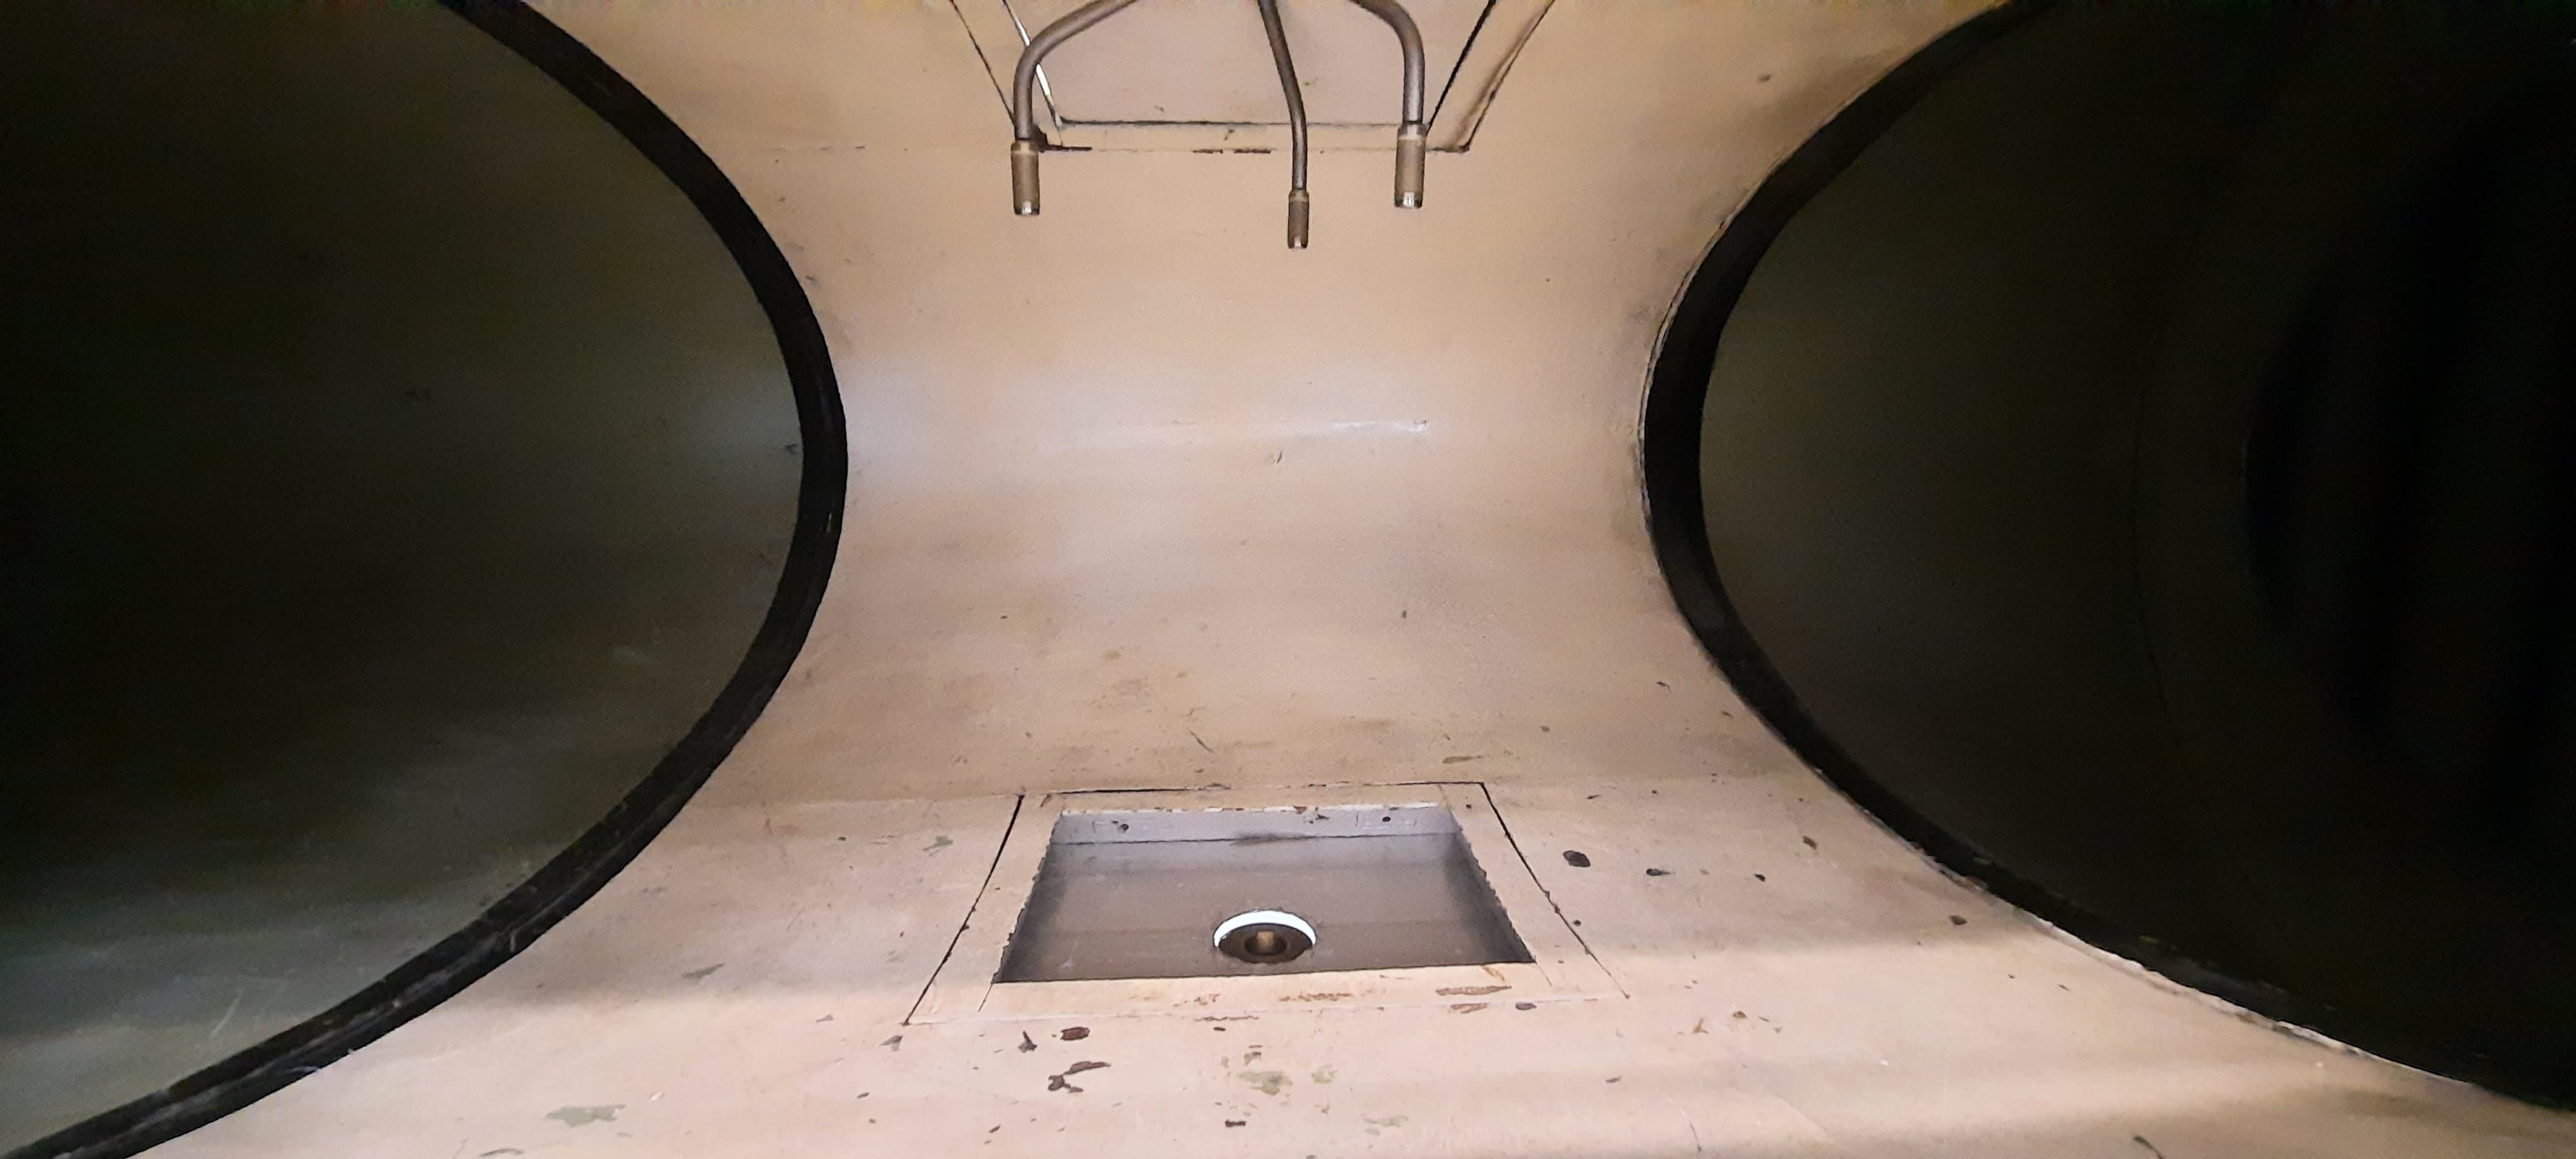
\includegraphics[width=\textwidth]{Figuras/viento/tunelDeViento/zonaDeMedicion.jpg}}
    \end{minipage}
    \caption{En (a) se muestra la vista lateral izquierda de la zona de medición, en (b) se muestran los álabes instalados en una de las esquinas en la parte derecha de la zona de medición, en (c) una vista frontal de la zona de medición.}
    \label{fig:tunelInterno}
\end{figure}

En la Figura \ref{fig:protectoresAuditivos} se muestran los protectores auditivos necesarios para trabajar con el túnel de viento. Debido a que el motor y el flujo de aire dentro del túnel producen un alto nivel de ruido, estos protectores son indispensables para garantizar la seguridad laboral y proteger la audición del personal. En la Figura \ref{fig:mesaDeTrabajo} se muestra la mesa de trabajo, que está equipada con una PC, una rosa de los vientos. Además, la mesa cuenta con conexión a internet mediante un switch, lo cual facilita la transferencia de datos y la comunicación en tiempo real durante los ensayos.

\begin{figure}[H]
    \centering
    \begin{minipage}[b]{0.45\textwidth}
        % \centering
        \subcaptionbox{\label{fig:protectoresAuditivos}}{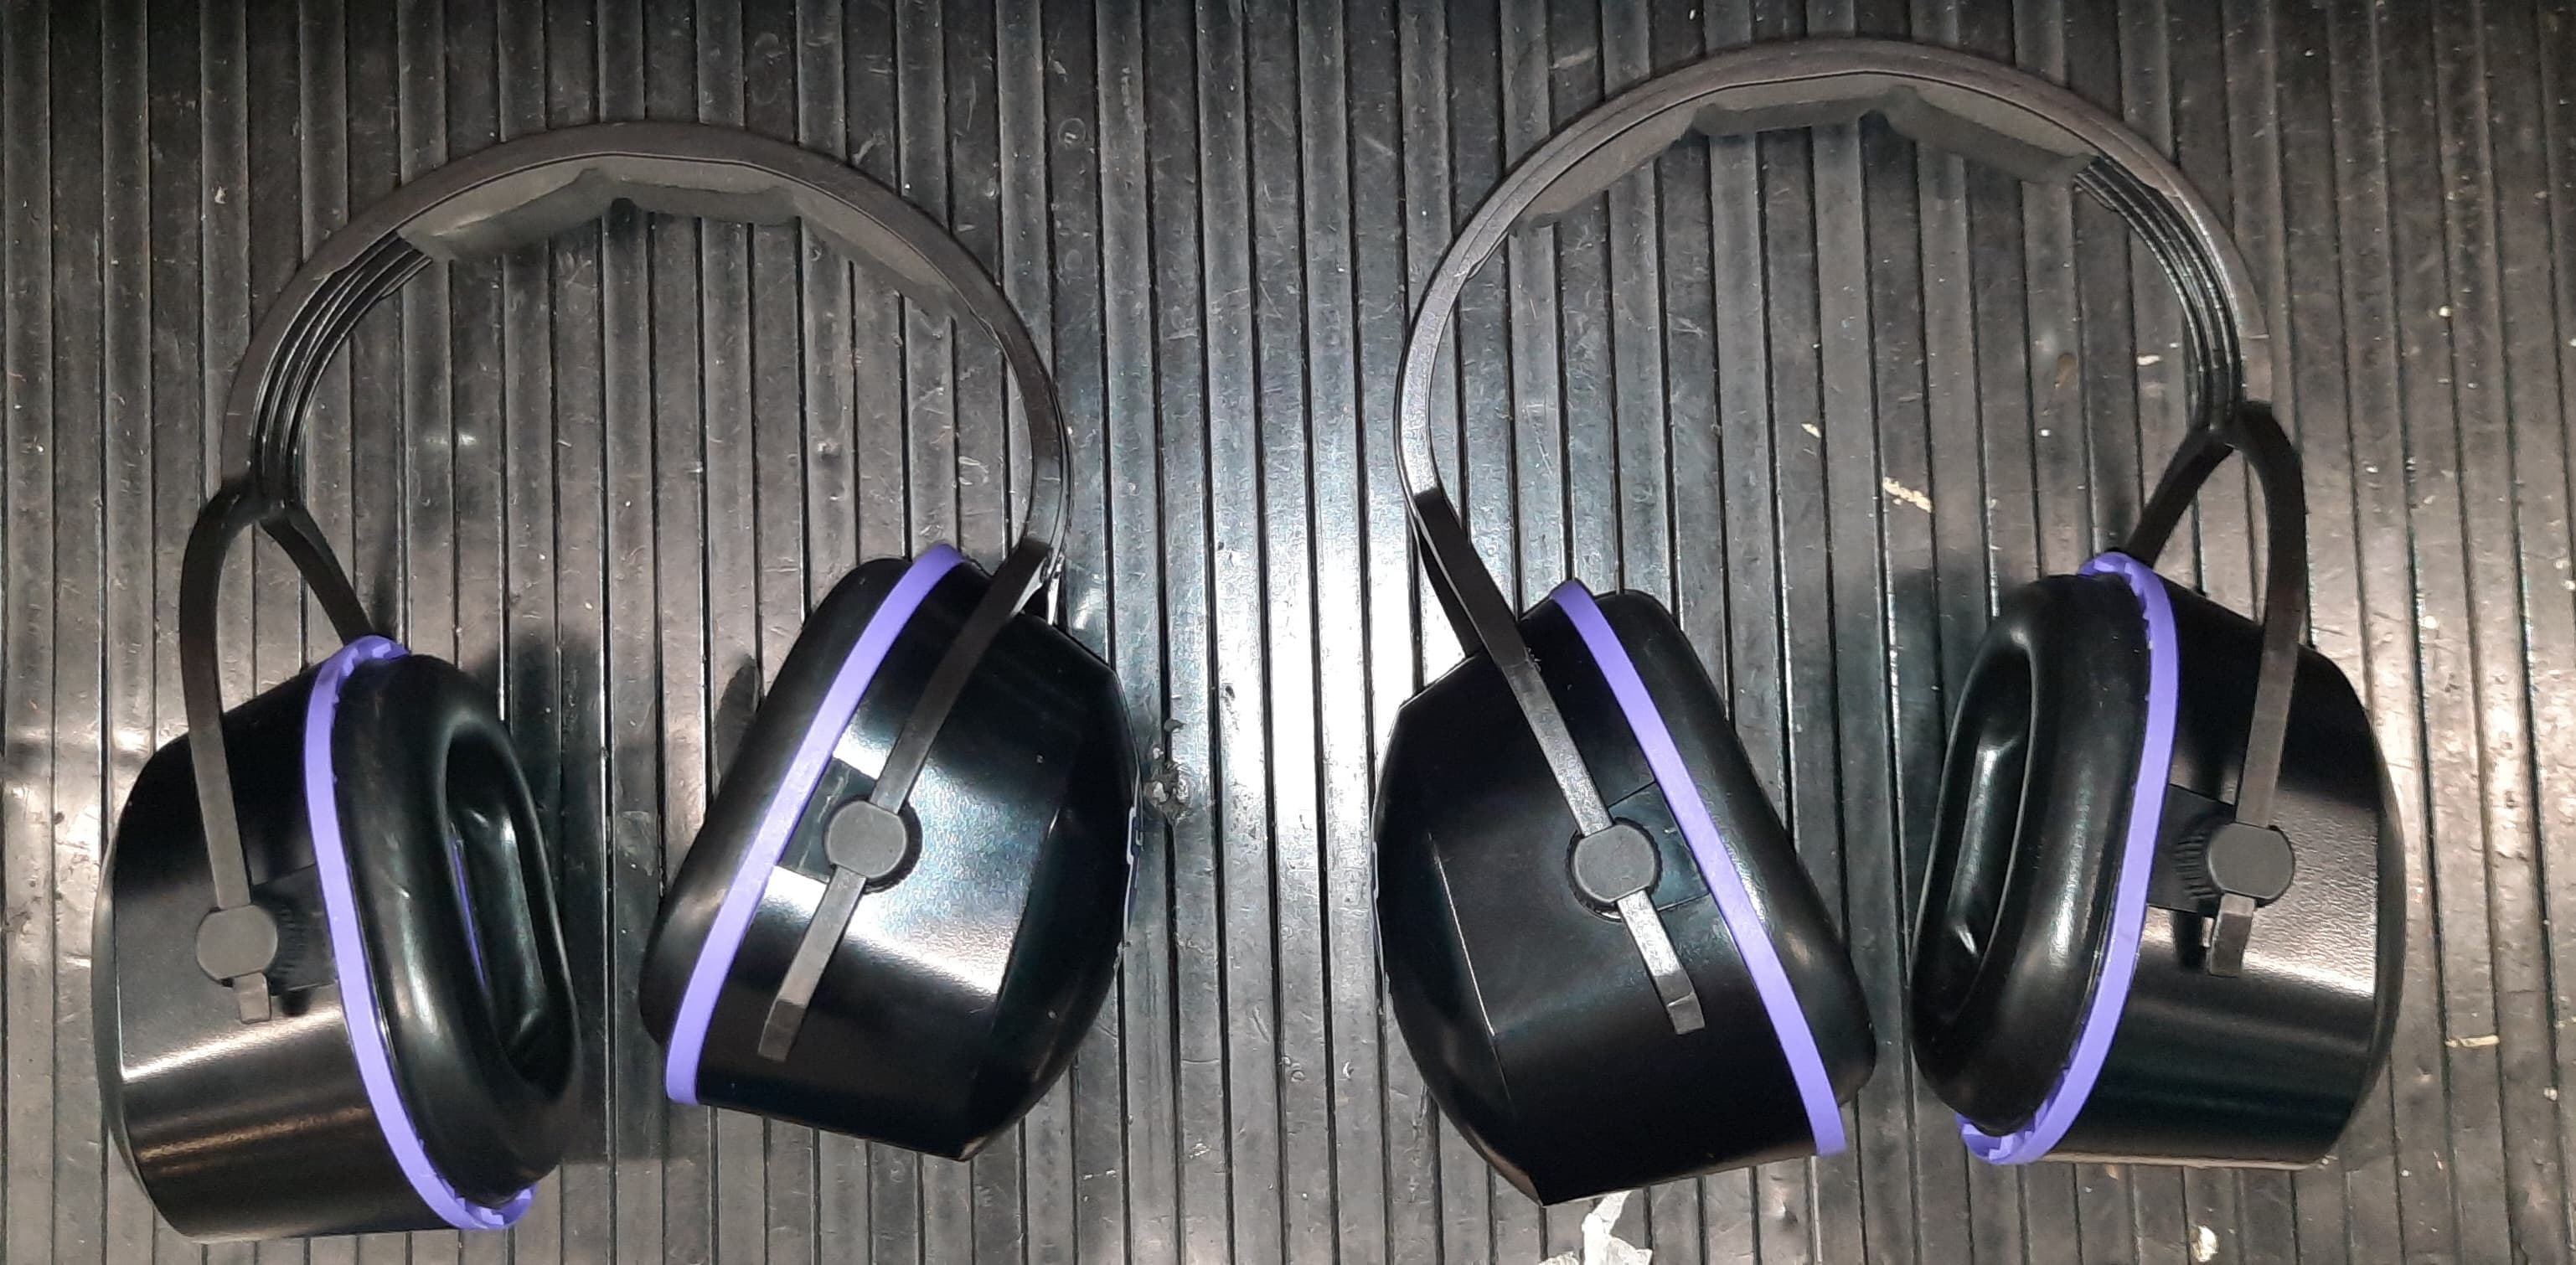
\includegraphics[width=\textwidth]{Figuras/viento/tunelDeViento/protectoresAuditivos.jpg}}
    \end{minipage}
    \hspace{1em} % Espacio vertical entre las filas
    \begin{minipage}[b]{0.45\textwidth}
        \subcaptionbox{\label{fig:mesaDeTrabajo}}{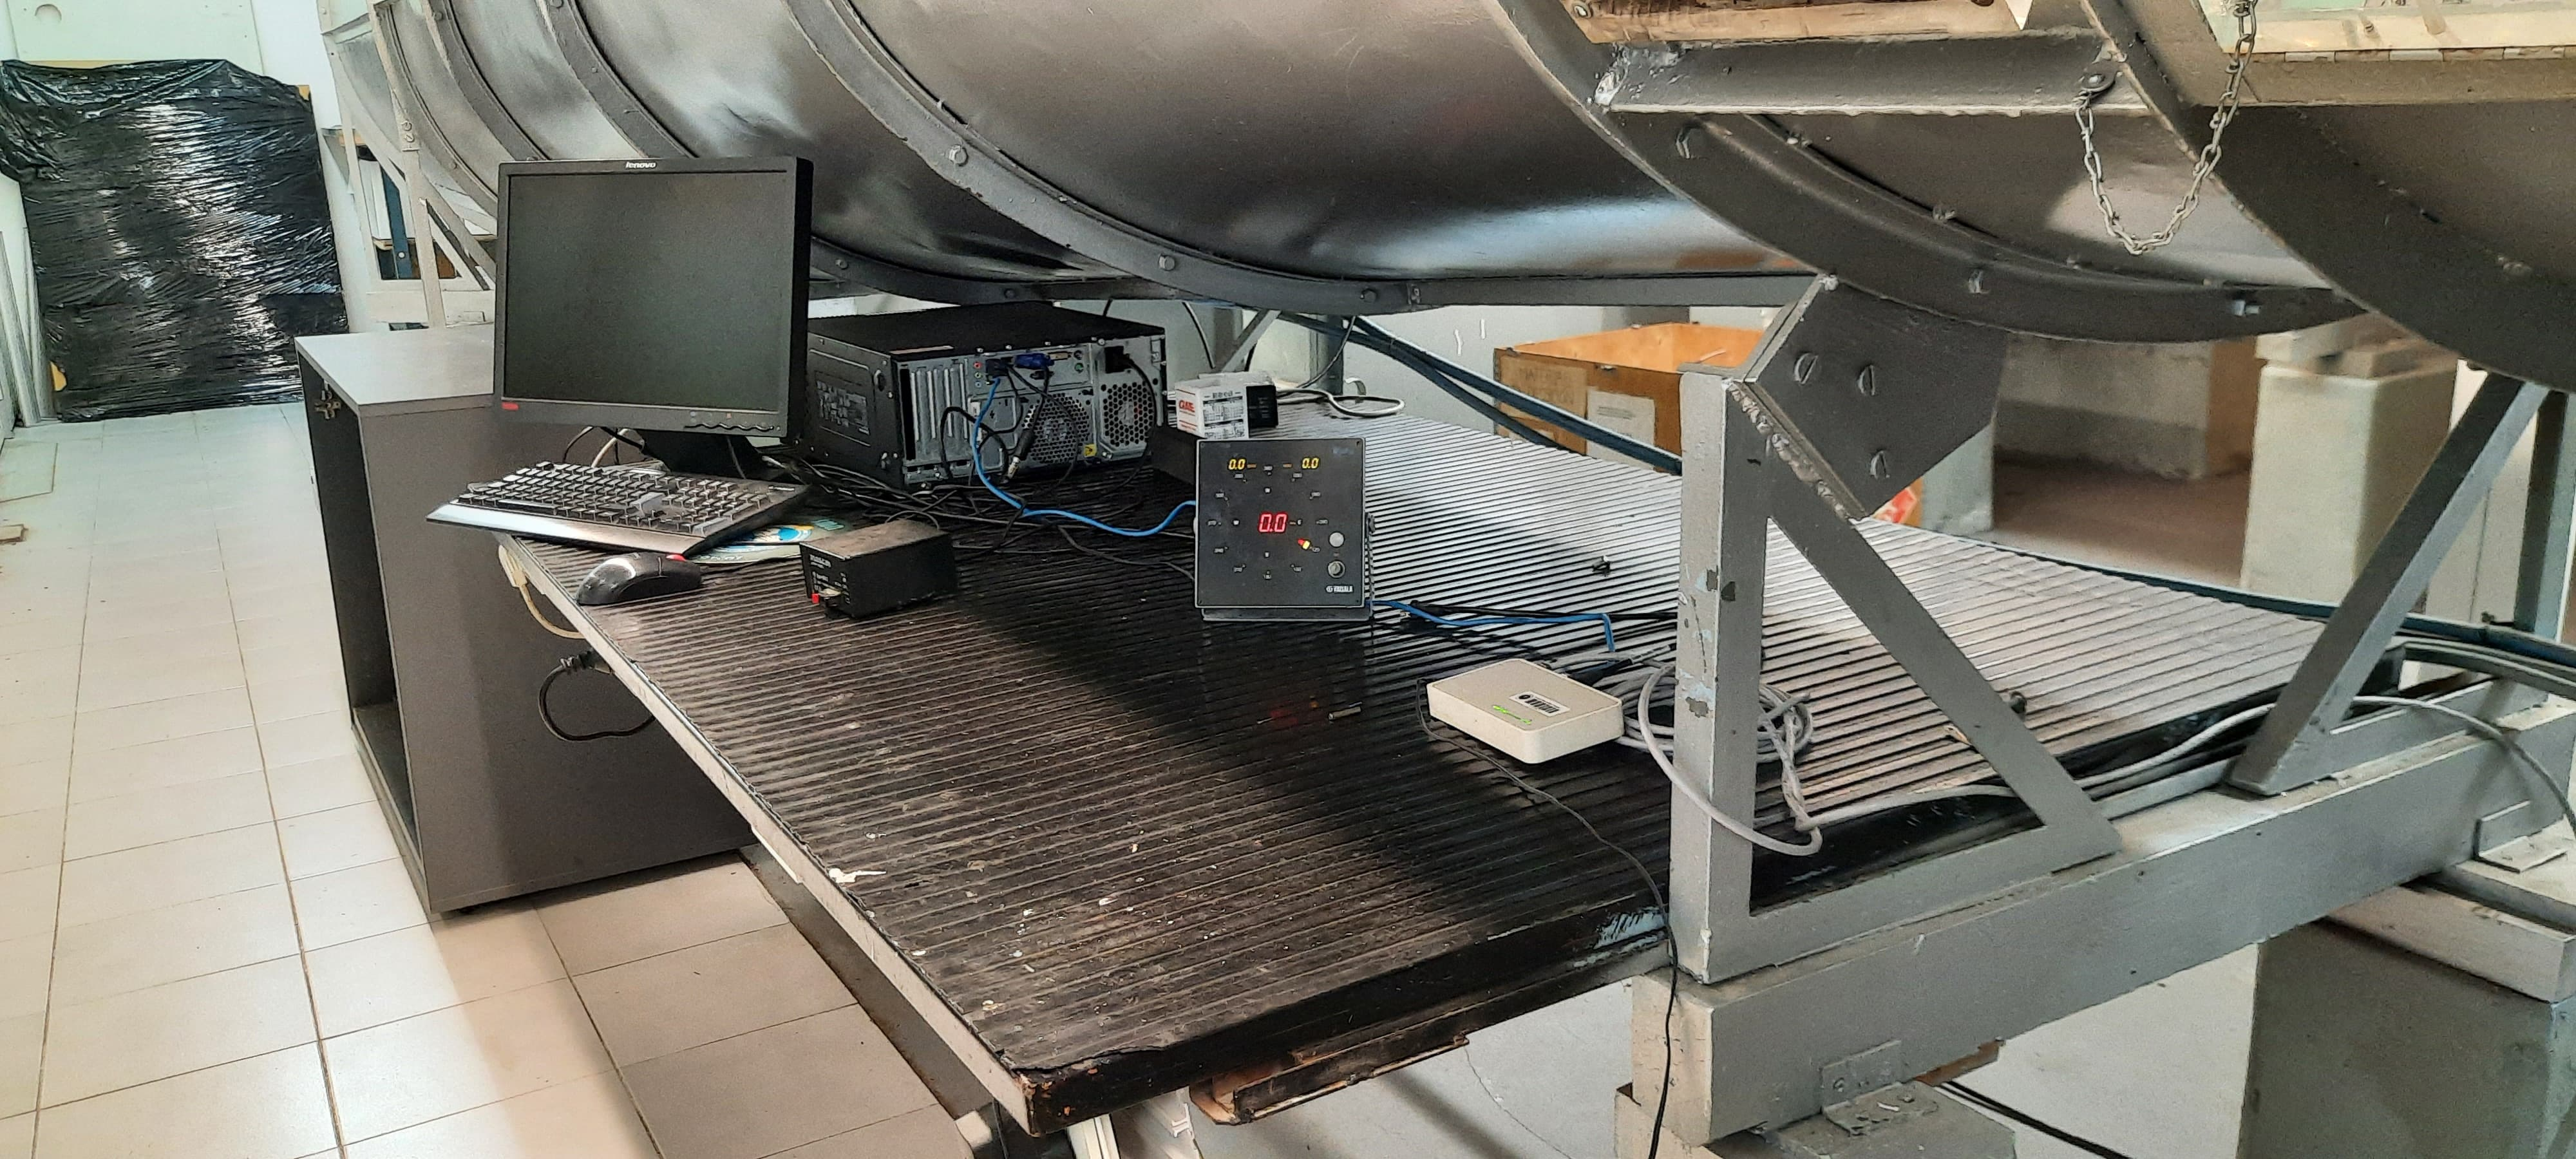
\includegraphics[width=\textwidth]{Figuras/viento/tunelDeViento/mesaDeTrabajo.jpg}}
    \end{minipage}  
    \caption{En (a) se muestra los protectores auditivos y en (b) se muestra la mesa de trabajo.}
    \label{fig:utensiliosParaTunel}
\end{figure}    

En las Figuras \ref{fig:motorLateralIzqui} y \ref{fig:motorLateralDerecha} se muestra el motor de corriente continua de \SI{16}{\kilo\watt} y 1800 rpm, el cual permite alcanzar velocidades de viento en el rango estimado de \SI{1}{\meter\per\second} a \SI{25}{\meter\per\second}. Este cuenta con cuatro poleas con sus respectivas correas para realizar la transmisión de movimiento, como se muestra en las Figuras \ref{fig:transmisionSuperior} y \ref{fig:transmisionInferior}, las poleas inferiores van conectadas al eje del motor y las poleas superiores van conectadas a un rodamiento sobre un eje superior. En la Figura \ref{fig:heliceMotor} se muestra el otro extremo del eje superior, conectado a la hélice diseñada en madera. Parte de la limitación de la velocidad del túnel se debe a la alineación de las poleas y al mantenimiento de las correas.



\begin{figure}[H]
    \centering
    \begin{minipage}{0.3\textwidth}
        \centering
        \subcaptionbox{\label{fig:motorLateralIzqui}}{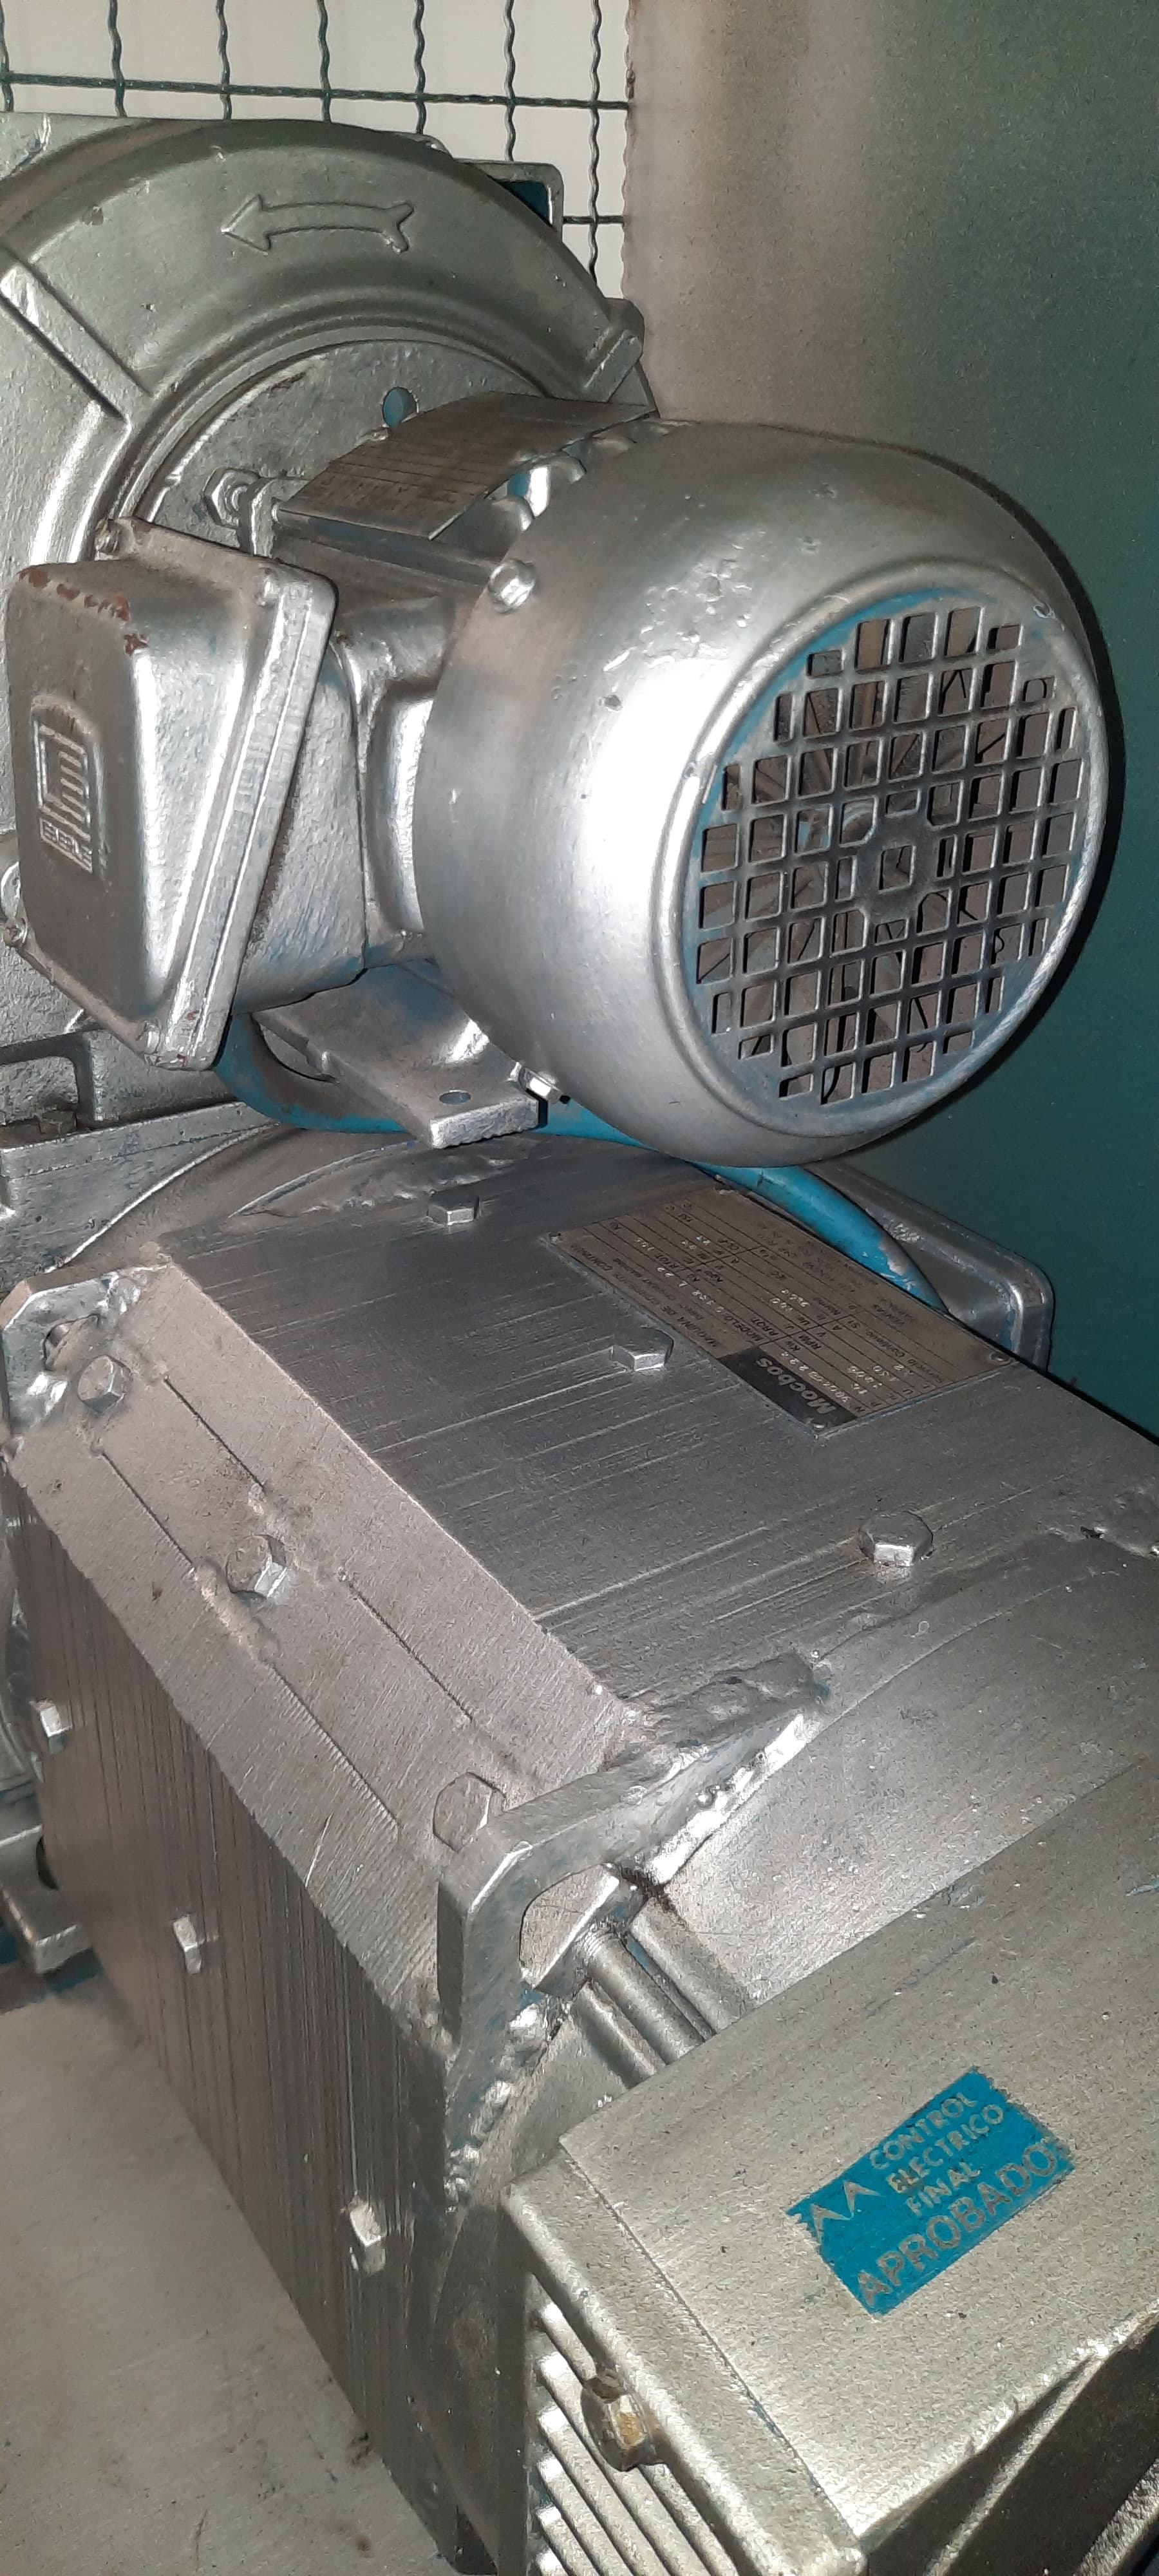
\includegraphics[width=0.8\textwidth]{Figuras/viento/tunelDeViento/motorLateralIzqui.jpg}}
    \end{minipage}
    \begin{minipage}{0.3\textwidth}
        \centering
        \subcaptionbox{\label{fig:motorLateralDerecha}}{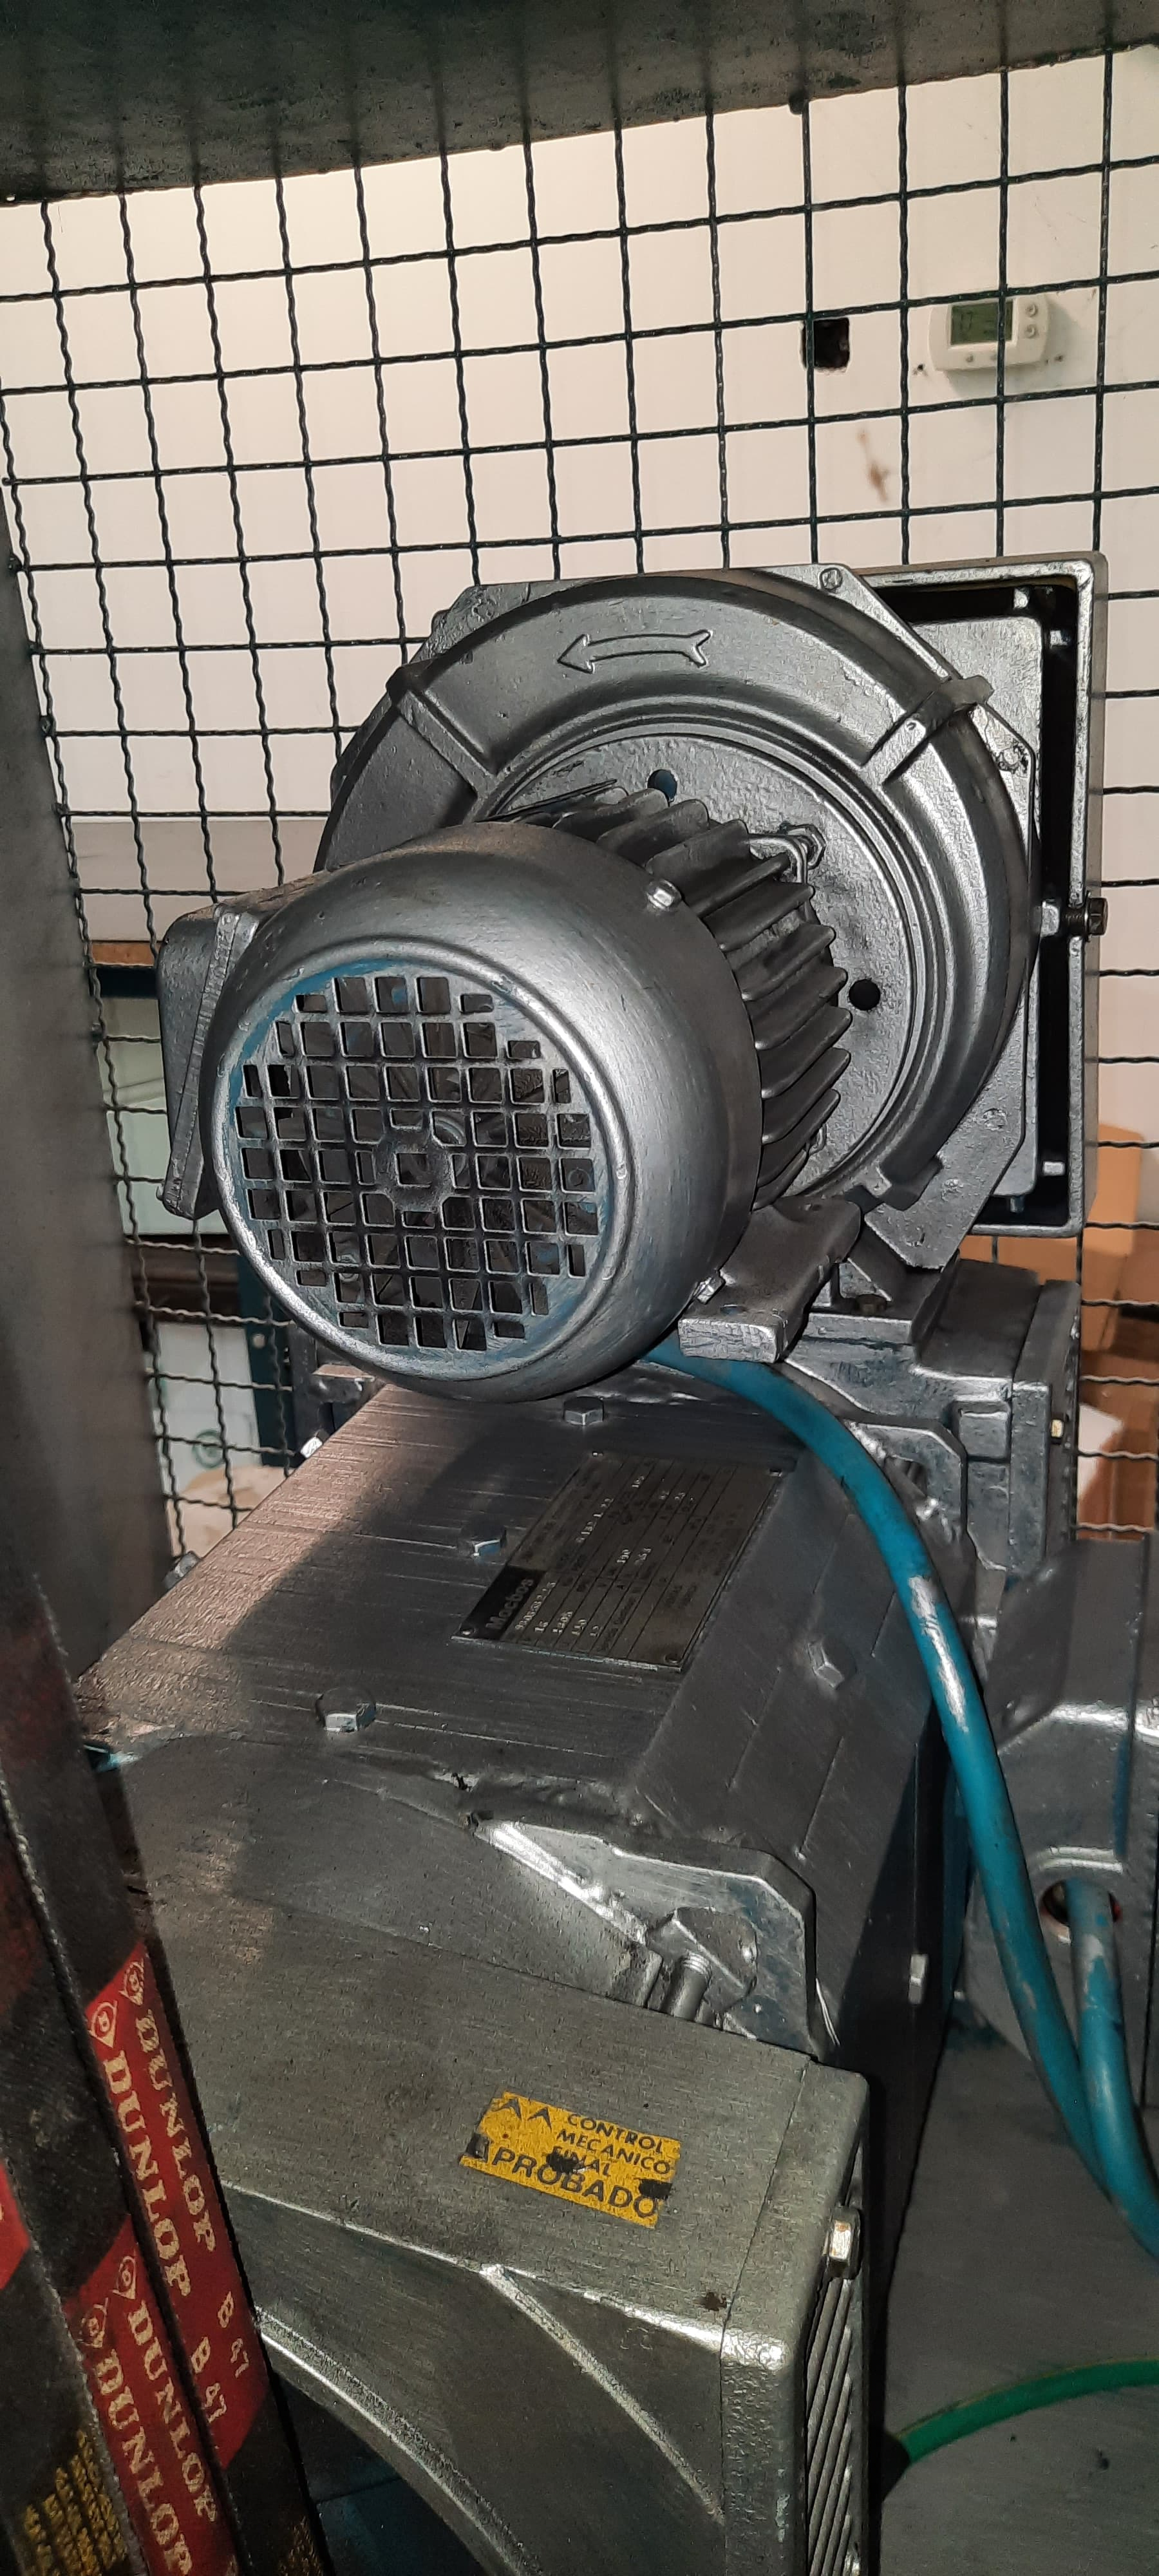
\includegraphics[width=0.8\textwidth]{Figuras/viento/tunelDeViento/motorLateralDerecha.jpg}}
    \end{minipage}
    \begin{minipage}{0.3\textwidth}
        \centering
        \subcaptionbox{\label{fig:transmisionSuperior}}{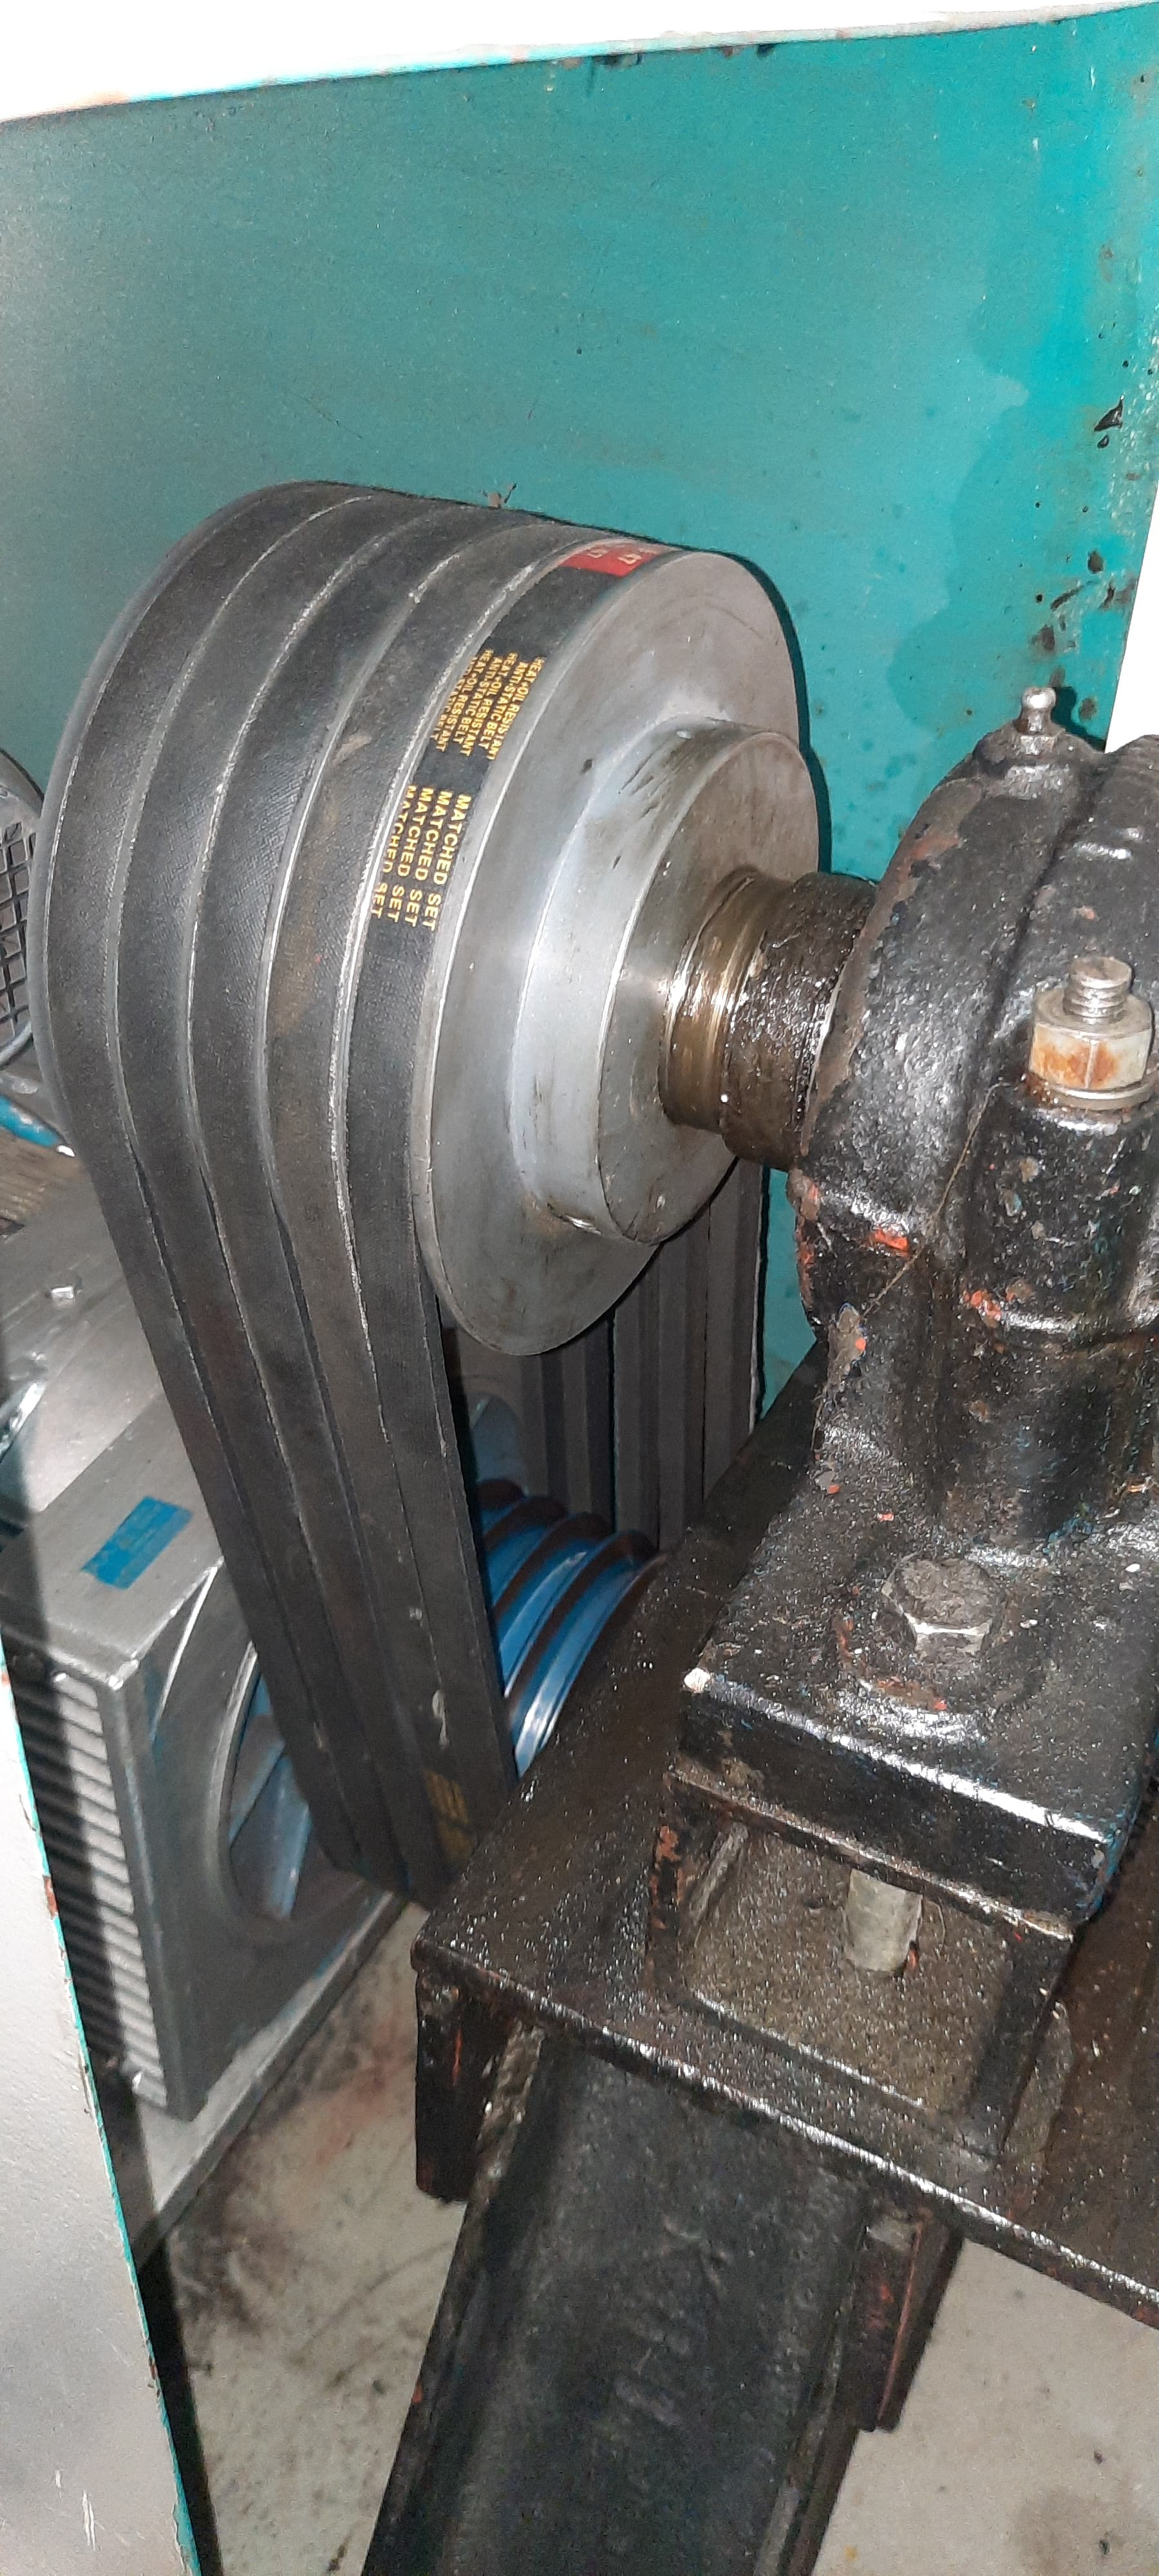
\includegraphics[width=0.8\textwidth]{Figuras/viento/tunelDeViento/transmisionSuperior.jpg}}
    \end{minipage}
    
    \vspace{1em} % Espacio vertical entre las filas
    
    \begin{minipage}{0.4\textwidth}
        \centering
        \subcaptionbox{\label{fig:transmisionInferior}}{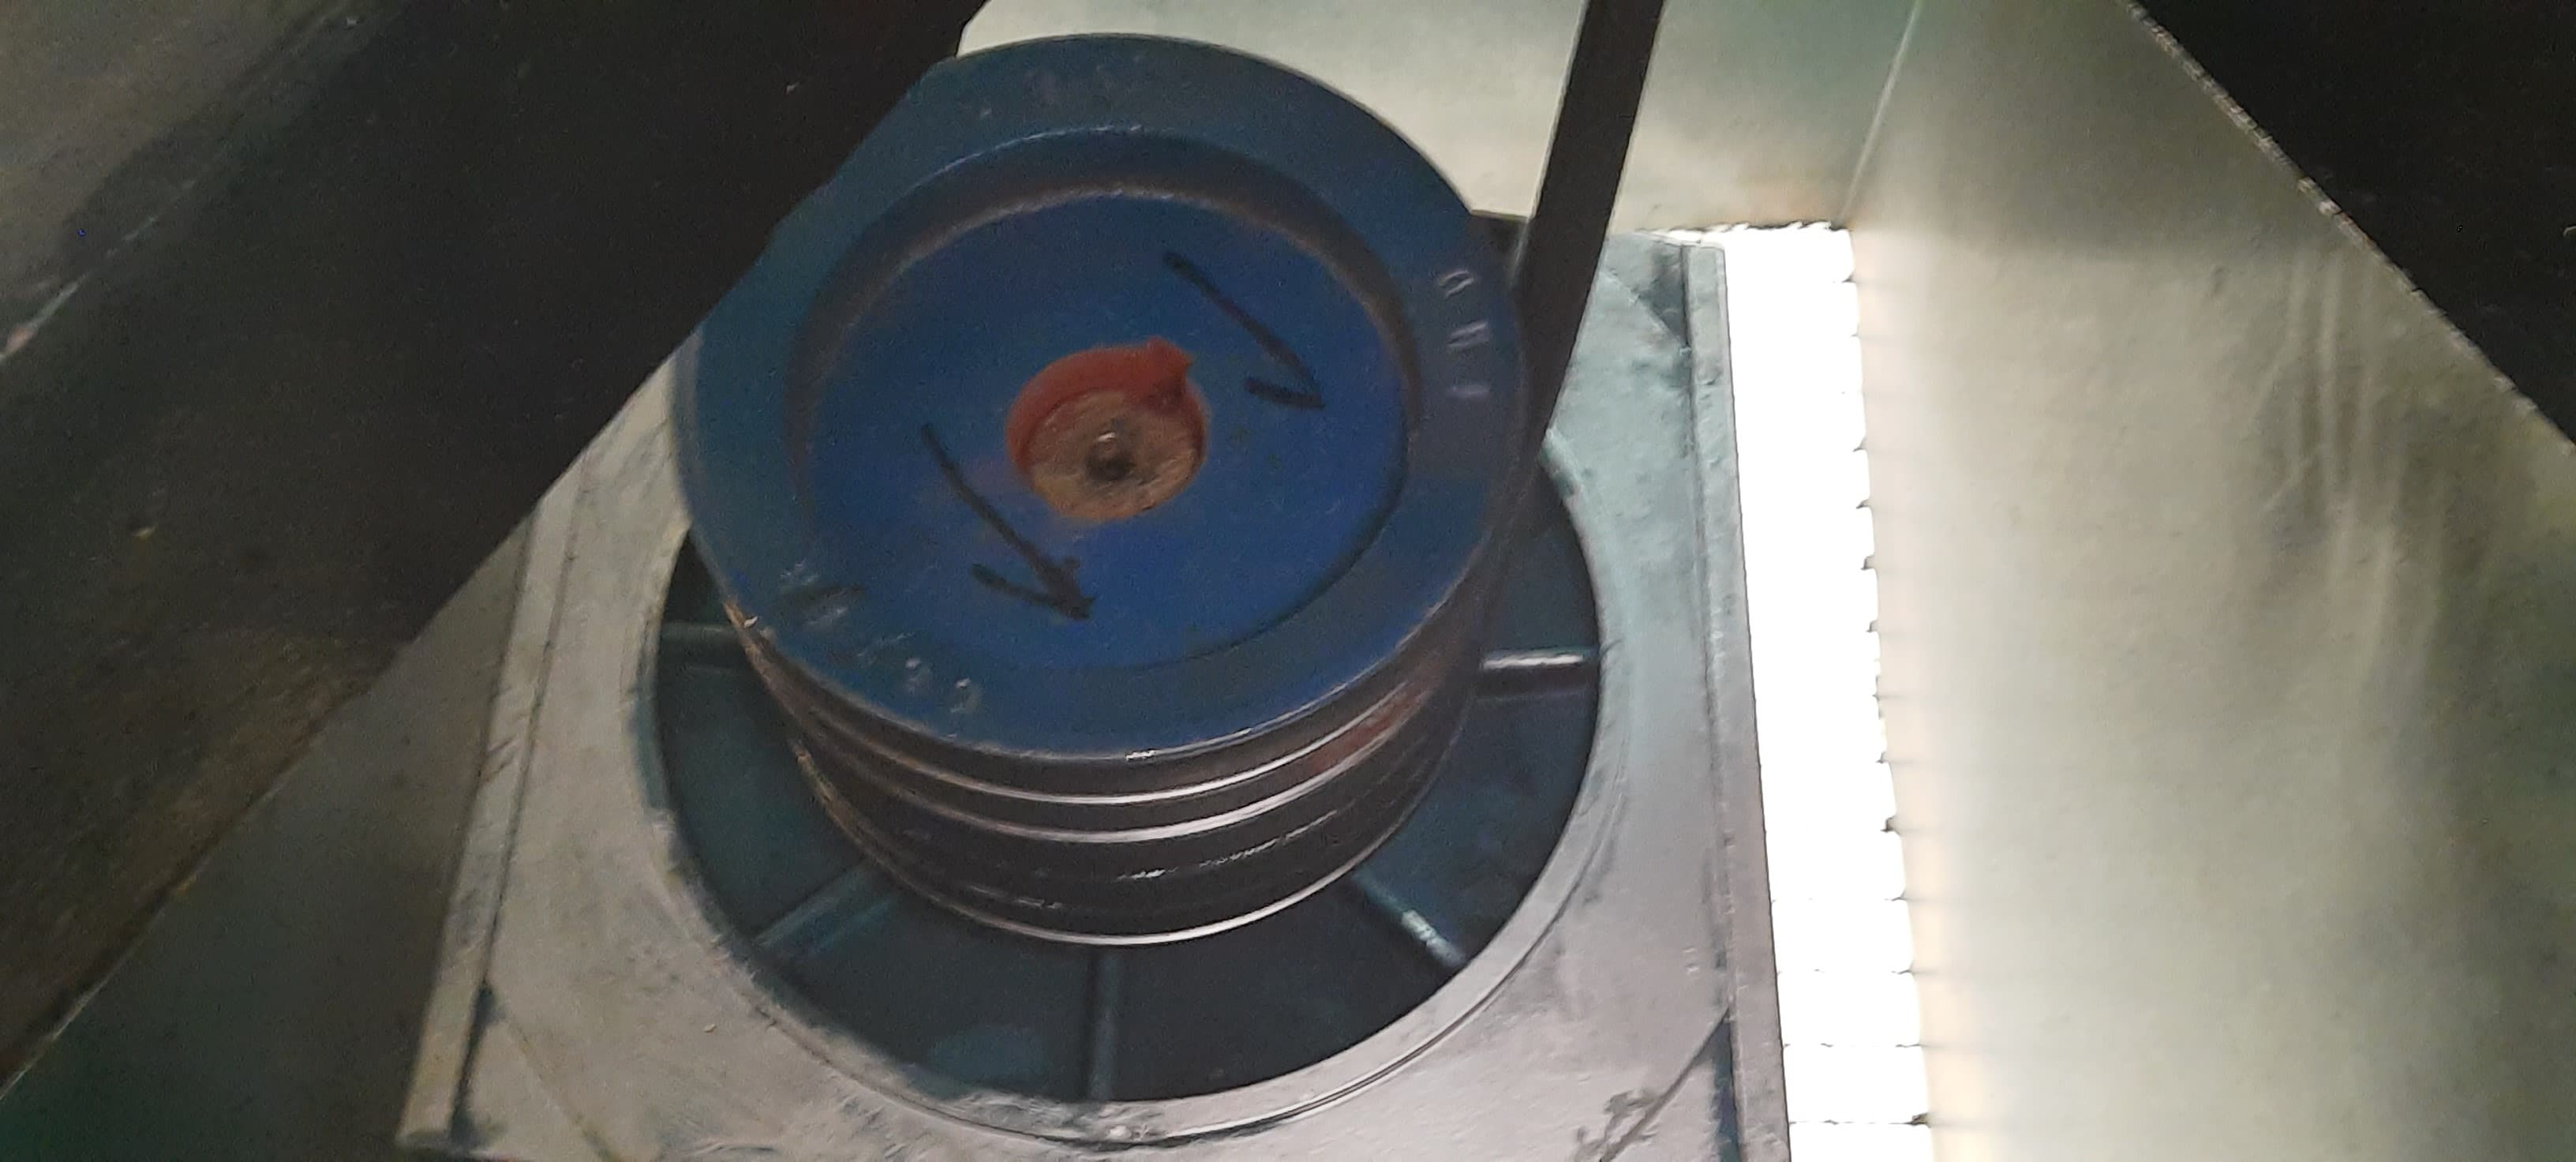
\includegraphics[width=1\textwidth]{Figuras/viento/tunelDeViento/poleaInferior.jpg}}
    \end{minipage}
    \hspace{2em}
    \begin{minipage}{0.4\textwidth}
        \centering
        \subcaptionbox{\label{fig:heliceMotor}}{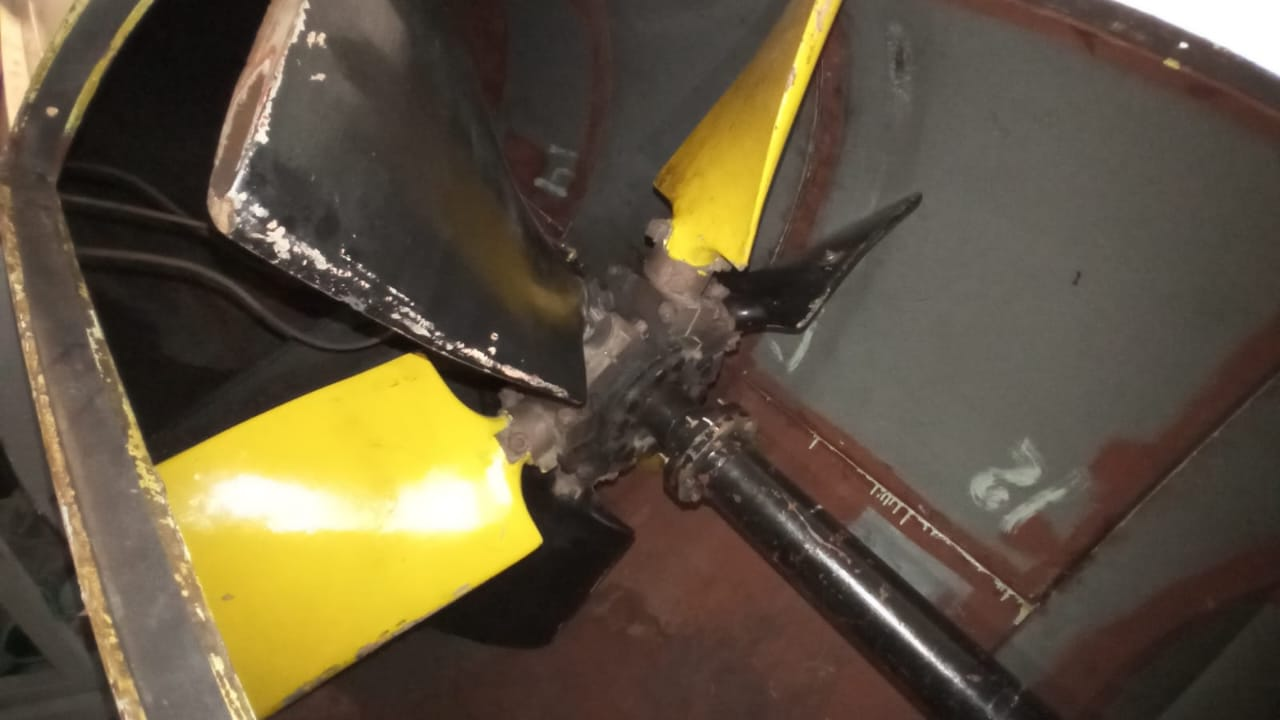
\includegraphics[width=1.2\textwidth]{Figuras/viento/tunelDeViento/heliceMotor.jpg}}
    \end{minipage}
    \caption{En (a) se muestra la vista lateral izquierda del motor, en (b) la vista lateral derecha, en (c) se muestra las correas conectadas a la polea superior que va al eje de la hélice, en (d) se muestra el eje del motor conectado a la polea inferior y las correas y en (e) se muestra la hélice del túnel.}
    \label{fig:motorPolea}
\end{figure}

 En la Figura \ref{fig:tableroTunel} se muestra el panel de control manual, que cuenta con dos botones, uno para iniciar y otro para detener el motor. La potencia del motor que varía la velocidad del viento dentro del túnel se regula manualmente mediante dos potenciómetros lineales: P1 de \SI{1}{\kilo\ohm} y P2 de \SI{500}{\ohm}. Además, dispone de dos medidores que indican el nivel de tensión suministrada al motor. En la Figura \ref{fig:variadorDeVelocidadMotor} se puede observar el circuito de electrónica de potencia del variador que controla el túnel de viento. El variador recibe tensión trifásica, la cual se rectifica y se convierte en corriente continua para alimentar el motor del túnel.

\begin{figure}[H]
    \centering
    \begin{minipage}[b]{0.3\textwidth}
        % \centering
        \subcaptionbox{\label{fig:tableroTunel}}{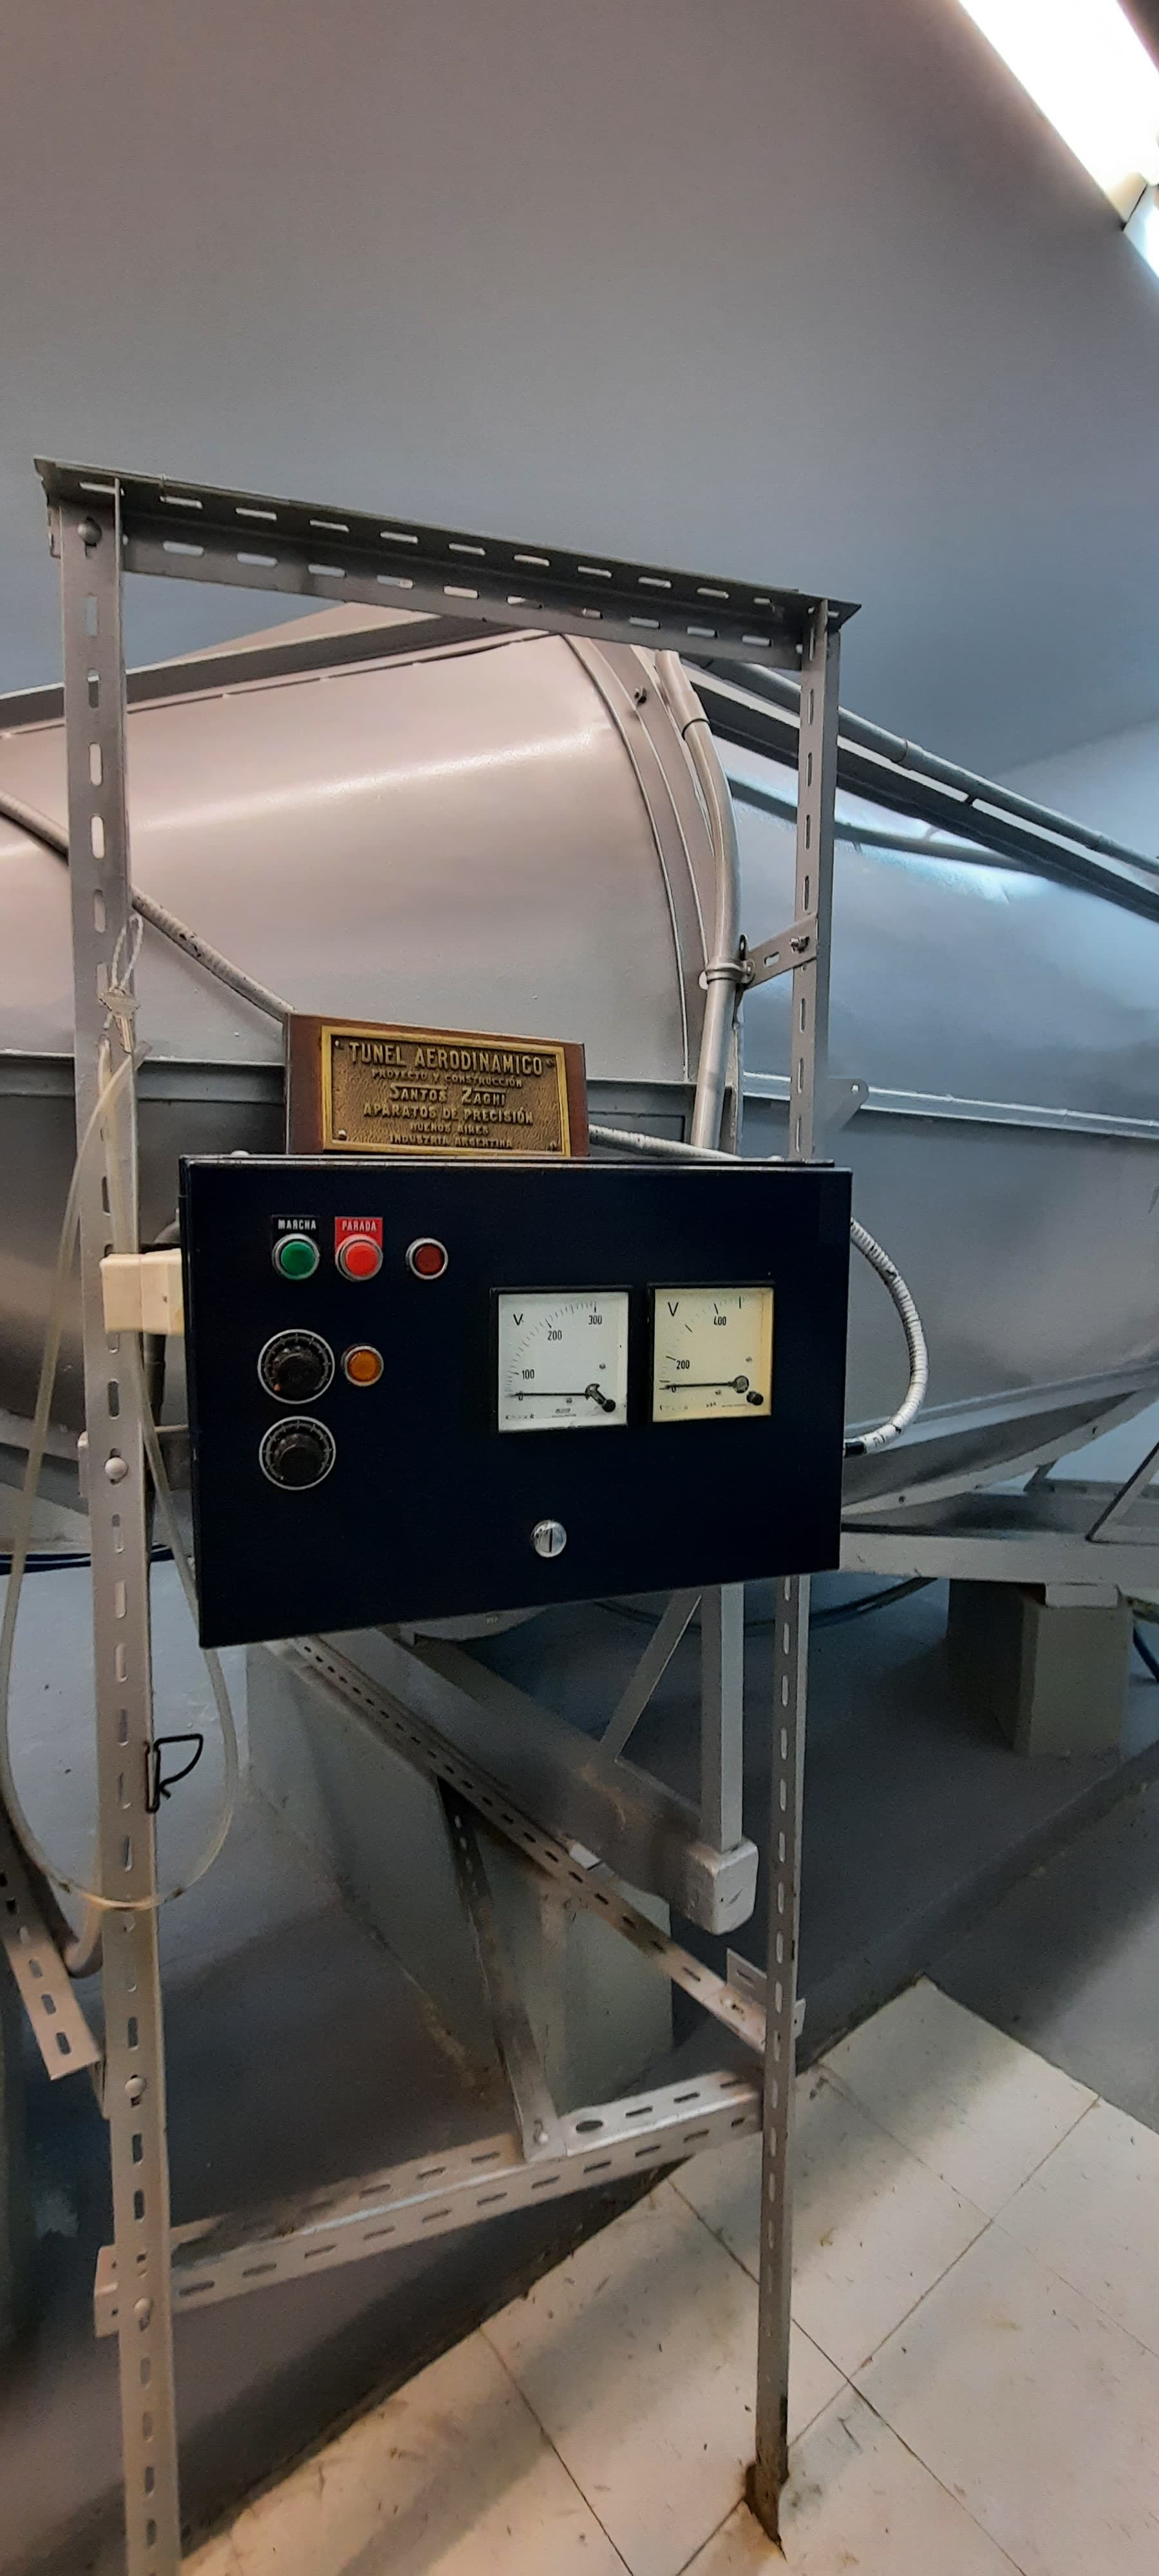
\includegraphics[width=\textwidth]{Figuras/viento/tunelDeViento/tableroTunel.jpg}}
    \end{minipage}
    \hspace{1em} % Espacio vertical entre las filas
    \begin{minipage}[b]{0.3\textwidth}
        \subcaptionbox{\label{fig:variadorDeVelocidadMotor}}{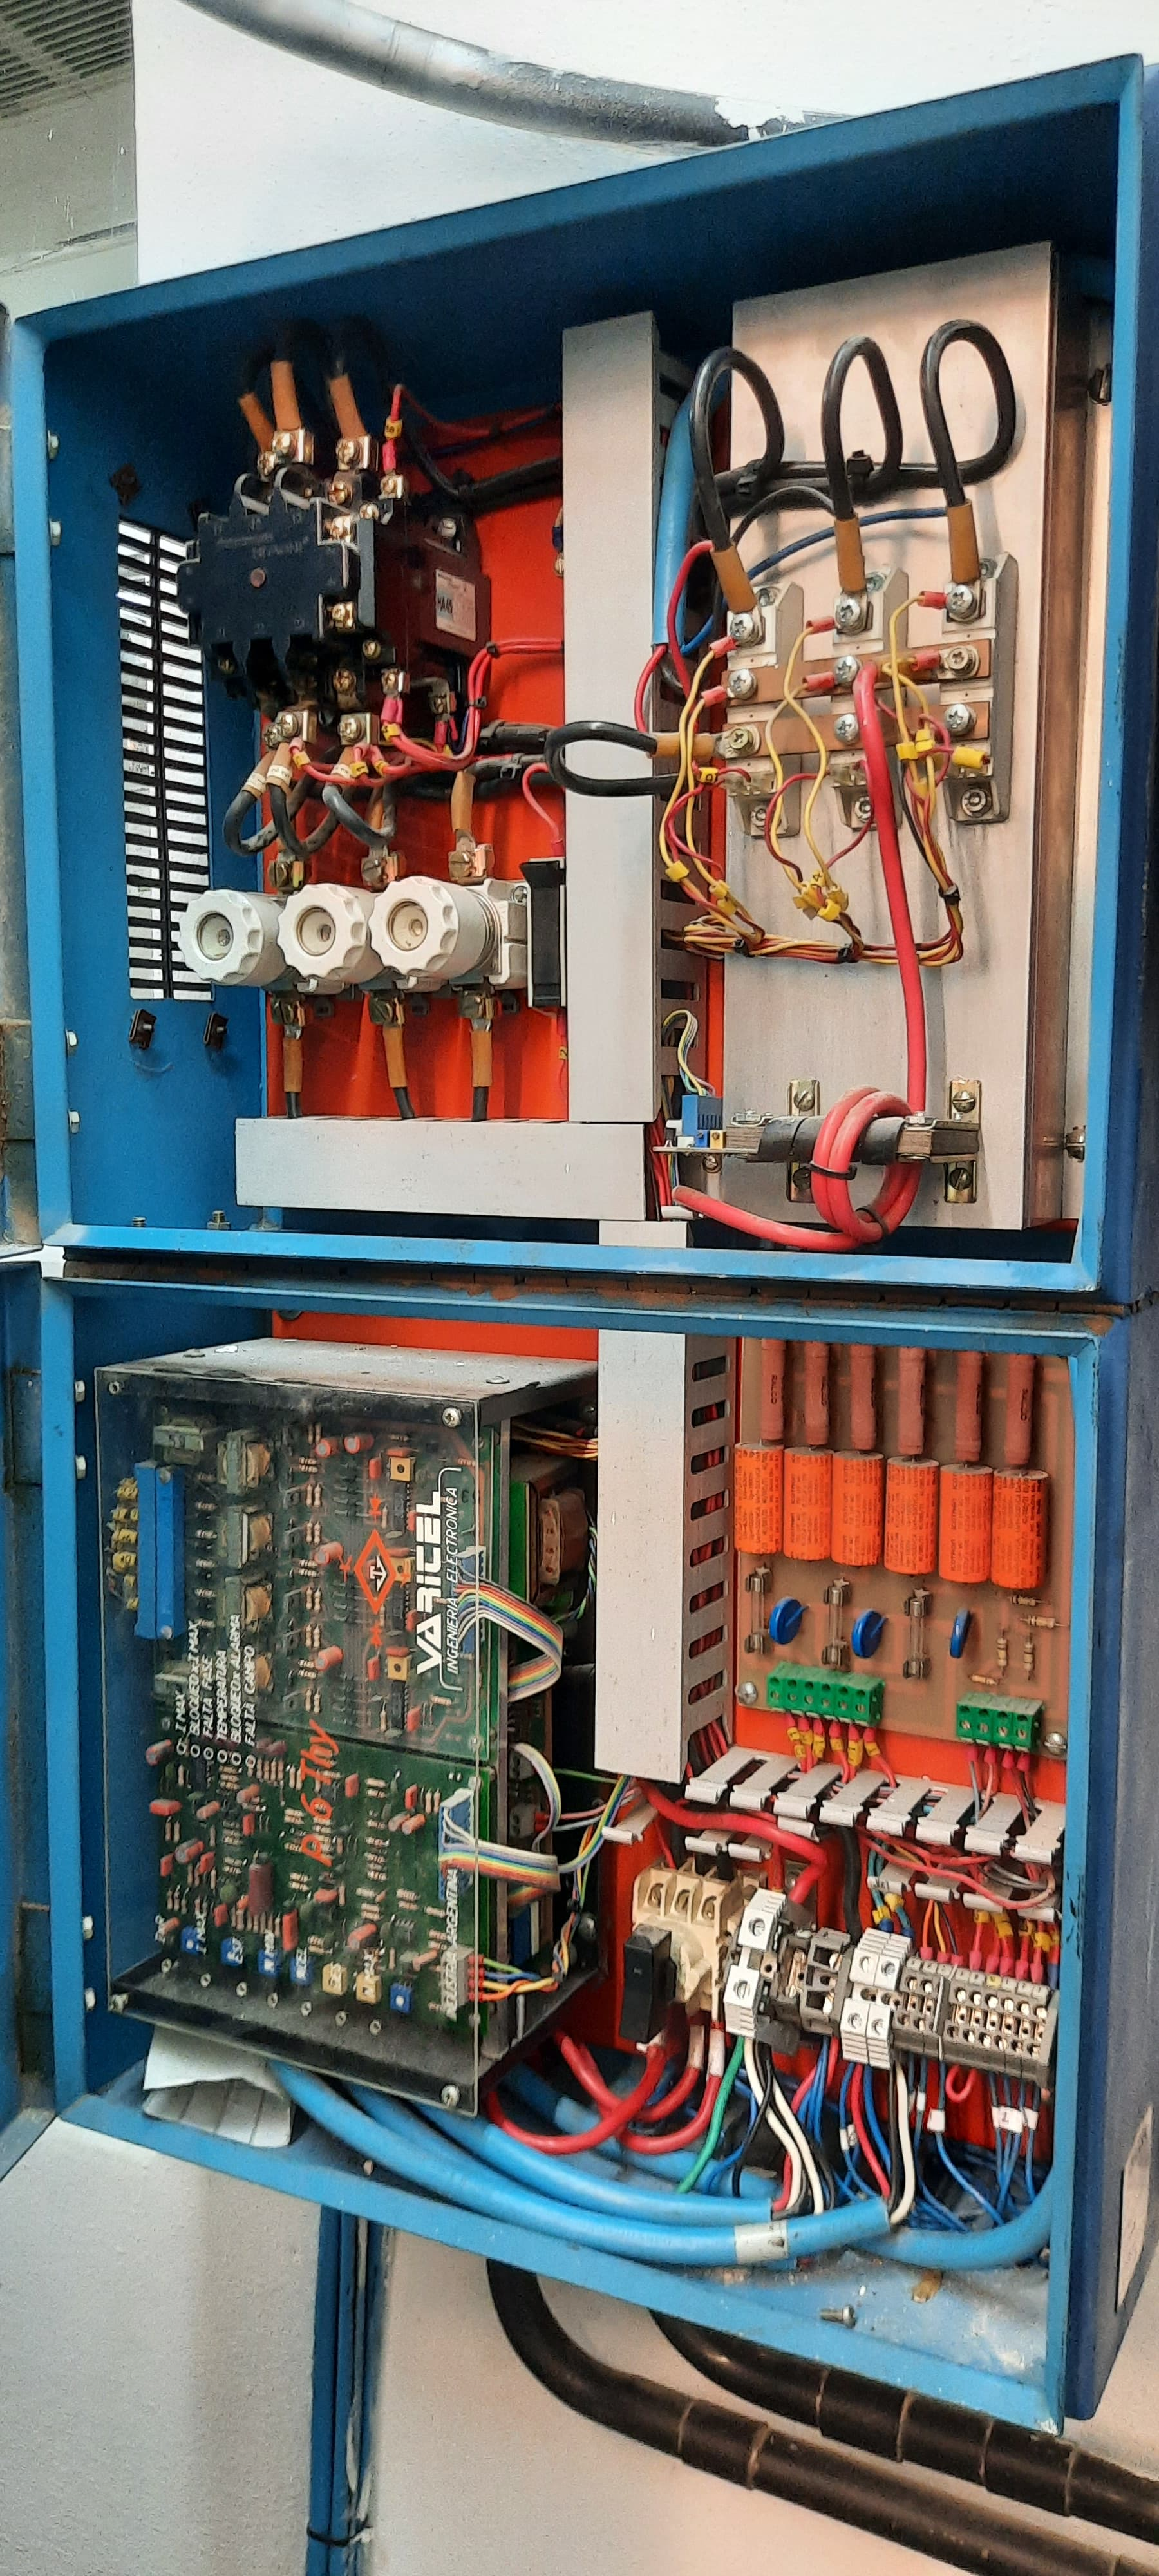
\includegraphics[width=\textwidth]{Figuras/viento/tunelDeViento/variadorDeVelocidadMotor.jpg}}
    \end{minipage}  
    \caption{En (a) se muestra el panel de control manual y en (b) el tablero eléctrico del variador de velocidad.}
    \label{fig:controlTunel}
\end{figure}    
